\RequirePackage{plautopatch} % pLaTeX / upLaTeX / LuaTeX-ja の不具合修正など
\documentclass[a4paper,10pt]{ltjsarticle}
\renewcommand{\baselinestretch}{1.05}
\usepackage{luatexja}        % LuaTeX-ja で日本語を扱う

% -------------------------------
% フォント関連の設定
% -------------------------------
\usepackage{luatexja-fontspec}

% -------------------------------
% 数式・数理フォントパッケージ
% -------------------------------
\usepackage{amsmath}
\usepackage{amssymb}          % \mathbb などを使用可能に

% -------------------------------
% 図を生成するためのパッケージ
% -------------------------------
\usepackage{tikz}
\usepackage{pgfplots}
\pgfplotsset{compat=newest}

% -------------------------------
% よく使われるパッケージ群
% -------------------------------
\usepackage{geometry}
\usepackage{multicol}
\usepackage{titlesec}
\usepackage{tocloft}
\usepackage[compatibility=false]{caption}
\usepackage{flushend}
\usepackage{graphicx}
\usepackage{here}
\usepackage{multirow}
\usepackage{threeparttable}
\usepackage{tabularx}  % 重複削除済み
\usepackage{enumitem}
\usepackage{url}
\usepackage{subcaption}  % subfig の代わりにこれを使用
\usepackage{indentfirst}
\usepackage{booktabs}
\usepackage{siunitx}


% -------------------------------
% 用紙余白等の設定
% -------------------------------
\geometry{
  top=20mm,
  bottom=20mm,
  left=20mm,
  right=20mm
}

\setlength{\baselineskip}{14pt}  % 行間

% -------------------------------
% タイトルやセクション見出しのフォーマット
% -------------------------------
\titleformat{\section}
  {\large\bfseries}
  {\thesection.}
  {1\zw}{}

\titleformat{\subsection}
  {\large\bfseries}
  {\thesubsection.}
  {1\zw}{}

\titleformat{\subsubsection}
  {\large\bfseries}
  {\thesubsubsection.}
  {1\zw}{}

\titlespacing*{\section}{0em}{1em}{1em}
\titlespacing*{\subsection}{0em}{1em}{1em}
\titlespacing*{\subsubsection}{0em}{1em}{1em}

% -------------------------------
% 目次の設定
% -------------------------------

\setcounter{tocdepth}{3}          % 目次の深さ
\makeatletter
\renewcommand{\numberline}[1]{#1.~}
\renewcommand{\cftsecleader}{\cftdotfill{\cftdotsep}}
\renewcommand{\cftsubsecleader}{\hfill}
\renewcommand{\cftsubsubsecleader}{\hfill}
\cftpagenumbersoff{subsection}
\cftpagenumbersoff{subsubsection}
% (例) section, subsection, subsubsection のインデントを調整
\cftsetindents{section}{0em}{5em}
\cftsetindents{subsection}{1em}{5em}
\cftsetindents{subsubsection}{1.5em}{5em}
\makeatother

% キャプション(図表の見出し)フォントサイズ設定
\DeclareCaptionFont{designatedFont}{\fontsize{10.5pt}{14pt}\selectfont}
\captionsetup{font=designatedFont}

% -------------------------------
% タイトル情報
% -------------------------------
% \title{サンプル論文タイトル}
% \author{山田 太郎}
% \date{\today}

% --- 表紙用追加パッケージ ---
\usepackage{xcolor}     % 色の指定
\usepackage{setspace}   % 行間設定

% --- タイトル作成のカスタマイズ ---
\makeatletter
\def\@maketitle{
\begin{flushright}
{\large \@date}  % 日付を右揃え
\end{flushright}
\begin{center}
{\LARGE \@title \par}  % タイトルを中央揃え
\end{center}
\begin{flushright}
{\large \@author}  % 著者を右揃え
\end{flushright}
\par\vskip 1.5em  % タイトル下の余白調整
}
\makeatother

% --- 表紙用の設定 ---
% 表紙変数の定義
\makeatletter
\newcommand{\programnumber}[1]{\def\thesis@programnumber{#1}}
\newcommand{\graduationyear}[1]{\def\thesis@graduationyear{#1}}
\newcommand{\japanesetitle}[1]{\def\thesis@japanesetitle{#1}}
\newcommand{\englishtitle}[1]{\def\thesis@englishtitle{#1}}
\newcommand{\studentname}[1]{\def\thesis@studentname{#1}}
\newcommand{\supervisor}[1]{\def\thesis@supervisor{#1}}
\newcommand{\institution}[1]{\def\thesis@institution{#1}}

% デフォルト値の設定
\programnumber{TB-07}
\graduationyear{令和6年度}
\japanesetitle{クロスレイヤシミュレータにおける\\無線LAN評価モデルの検討}
\englishtitle{A Study of a Wireless LAN Evaluation Model\\in a Cross-Layer Simulator}
\studentname{下沢 亮太郎}
\supervisor{設樂 勇}
\institution{東京都立産業技術高等専門学校}

% 表紙ページの作成コマンド
\newcommand{\makecoverpage}{
  \begin{titlepage}
    \newgeometry{top=30mm, bottom=30mm, left=20mm, right=20mm}
    \thispagestyle{empty}
    {\large 発表プログラム番号\quad \thesis@programnumber}
    \begin{center}
      \vspace{25mm}
      {\LARGE \thesis@graduationyear\ 卒業論文}

      \vspace{35mm}
      {\huge \thesis@japanesetitle}

      \vspace{25mm}
      {\huge \thesis@englishtitle}

      \vspace{50mm}
      {\huge \thesis@studentname}

      \vfill
      {{\large 指導教員}\qquad {\huge \thesis@supervisor}}

      \vspace{20mm}
      {\Large \thesis@institution}
    \end{center}
    \restoregeometry
  \end{titlepage}
  \setcounter{page}{1}
}
\makeatother

% 文書開始時に自動的に表紙を出力するための設定
\AtBeginDocument{\makecoverpage}

\begin{document}

\tableofcontents
\thispagestyle{empty}


\clearpage
\setcounter{page}{1}

% ******************************************************
% はじめに
% ******************************************************

\section{はじめに}
\subsection{背景}

近年,無線通信端末の利用者が急増し,多様な場所で無線通信システムが活用されており今後も利用の拡大と機能の高度化が見込まれる.一方で,無線通信技術の進歩に伴いシステム自体はますます高機能化・複雑化している.

% しかし,研究開発の現場では各レイヤごとに検討が行われており,単一レイヤのみの評価では通信システム全体の性能を十分に把握することができない.

これまでの研究開発の現場では物理層,MAC層,ネットワーク層といった各レイヤごとに評価検討が行われてきた.しかし,無線LAN(Local Area Network)システムの高機能化・複雑化に伴い,単一レイヤのみ性能が高くなったとしても他レイヤの性能がボトルネックとなる問題が見られるようになった.
一例として,IEEE 802.11ac\cite{11std}では,MU-MIMO(Multi User Multiple Input Multiple Output)と呼ばれる高速化技術が使用されているが,端末数が増加すると通常のMIMOが有効となるケースもある.また,通信効率の観点から見るとMU-MIMOに比べて通常のMIMOの方が遥かに高効率である\cite{book1}.
この例のように,単一レイヤのみの性能向上では通信全体の性能を向上・評価できない場合がある.したがって,物理層から上位層まで考慮したクロスレイヤシミュレータの開発が求められている.

\subsection{目的}

本研究では,無線通信全体の品質を総合的に評価するために,実環境の電波伝搬特性を考慮した物理層とMAC(Medium Access Control)層が連携したシミュレータの開発の一環として,IEEE 802.11規格\cite{11std}に基づくCSMA/CA(Carrier Sense Multiple Access with Collision Avoidance,衝突回避機能付きキャリア感知多重アクセス)方式を用いたMAC層の動作に則った無線LANモデルを開発し,その精度を評価することを目指す.


% ******************************************************
% 関連する技術とその課題
% ******************************************************
\clearpage
\section{関連する技術とその課題}
\subsection{関連技術}
\subsubsection{CSMA/CA方式}


IEEE 802.11無線LAN(802.11 無線LAN)では,アクセス制御方式としてCSMA/CAが採用されている.802.11 無線LANの基本アクセス手順とされている自律分散制御(DCF : Distributed Coordination Function)では,各局がチャネルの使用状況を検査して自律的にパケット(フレーム)の送信タイミングを決定するが,その時のアクセス制御プロトコルとしてCSMA/CAを使用している.図\ref{fig:DCF}にDCFの概要,図\ref{CSMA/CA}にCSMA/CAの概要を示す.

フレームを送信していない無線局は,電波を送信していないため,Carrier(搬送波)の使用状況をSense(検出)し,一定時間未使用(Idle)であれば,Carrierを誰も使用していないと判断し,各端末がバックオフ時間としてランダムなスロット数を生成し,その時間だけ待った後に再度CSを行い,チャネルがIdleであれば送信を開始する.再度CSを行った結果,無線チャネルが使用中(Busy)であれば,フレームを送信できるまでバックオフ時間を持ち越す.複数の端末が同じスロット数となった場合には送信タイミングが同時になり,衝突が発生するため再送制御が必要となる.

また,無線通信ではCSMA/CD(Carrier Sense Multiple Access with Collision Detection)のように衝突を直接検知できないため,送信したフレームに対してACK(ACKnowledgment)フレームを受信することで,フレームが正常に受信されたかを確認する.ACKフレームを受信できなかった場合,フレームは正常に受信されなかったと判断し,再送処理を行う.

このため,たとえ周辺に同一チャネルを利用する無線セルが存在したとしてもCSMA/CAにより,無線セル間で同一チャネルを共有して通信できる.ただし,CSMA/CAでは,偶然同時にフレームを送信してしまう可能性,すなわちフレーム同士が無線上で衝突してしまう可能性がある.衝突によって,フレームが正常に受信されなかった場合,パケットは再送されるが,バックオフ時間の増加がオーバーヘッドの増加に繋がり,スループットが低下する.

CSMA/CAでは,フレームの送信を試みようとするそれぞれの無線局が事前にキャリアセンス(CS : Carrier Sense)を行い無線チャネルの使用状況を確認し,他の無線局による送信が行われている間,送信を見合わせる(送信待機)ことによって,衝突を可能な限り回避する.図\ref{fig:CS_level}にキャリアセンスレベルの概要を示す.無線LANにおいてキャリアセンスレベルは-62\,dBmと規定されており,キャリア・センス・エリア内からの-62\,dBm以上の受信電力レベル(干渉源1)を検出した場合はチャネルが使用中(Busy)と判断し,送信を待機する.一方で-62\,dBm未満の受信電力レベルが(干渉源2)検出された場合はチャネルが未使用(Idle)と判断し,送信を開始する.


\begin{figure}[H]
  \centering
  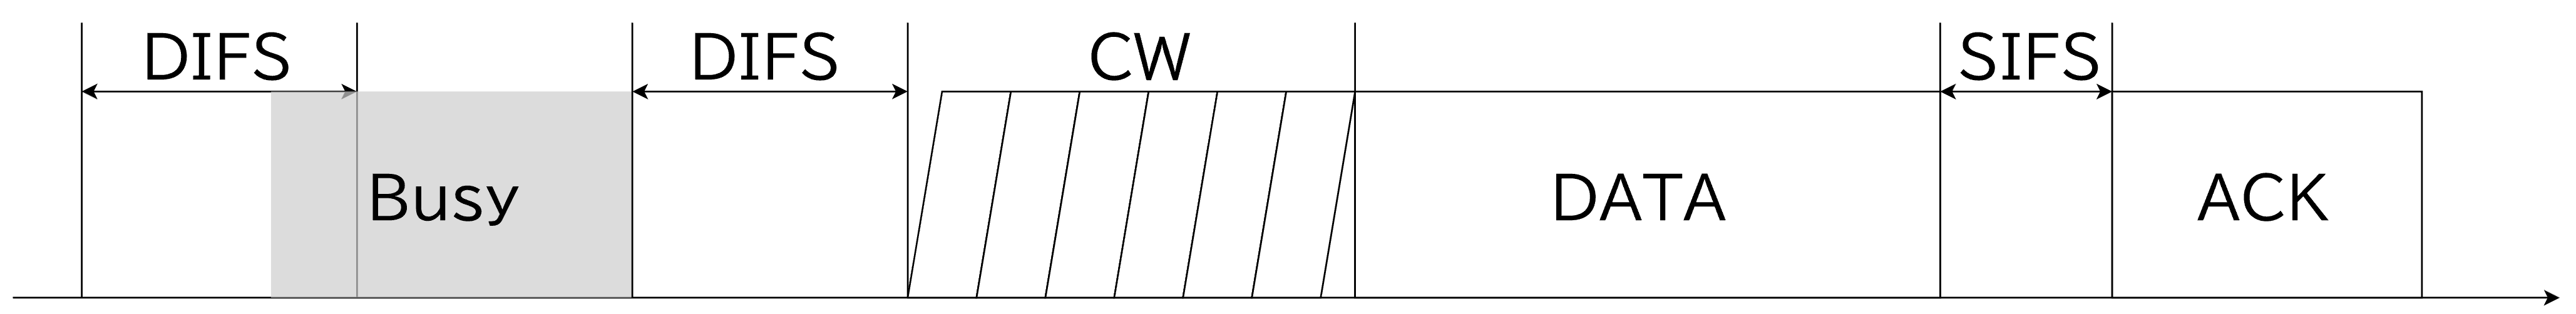
\includegraphics[width=0.8\textwidth]{./assets/DCF.png}
  \caption{DCF}
  \label{fig:DCF}

\end{figure}


\begin{figure}[H]
  \centering

  \begin{subfigure}{\textwidth}
    \centering
    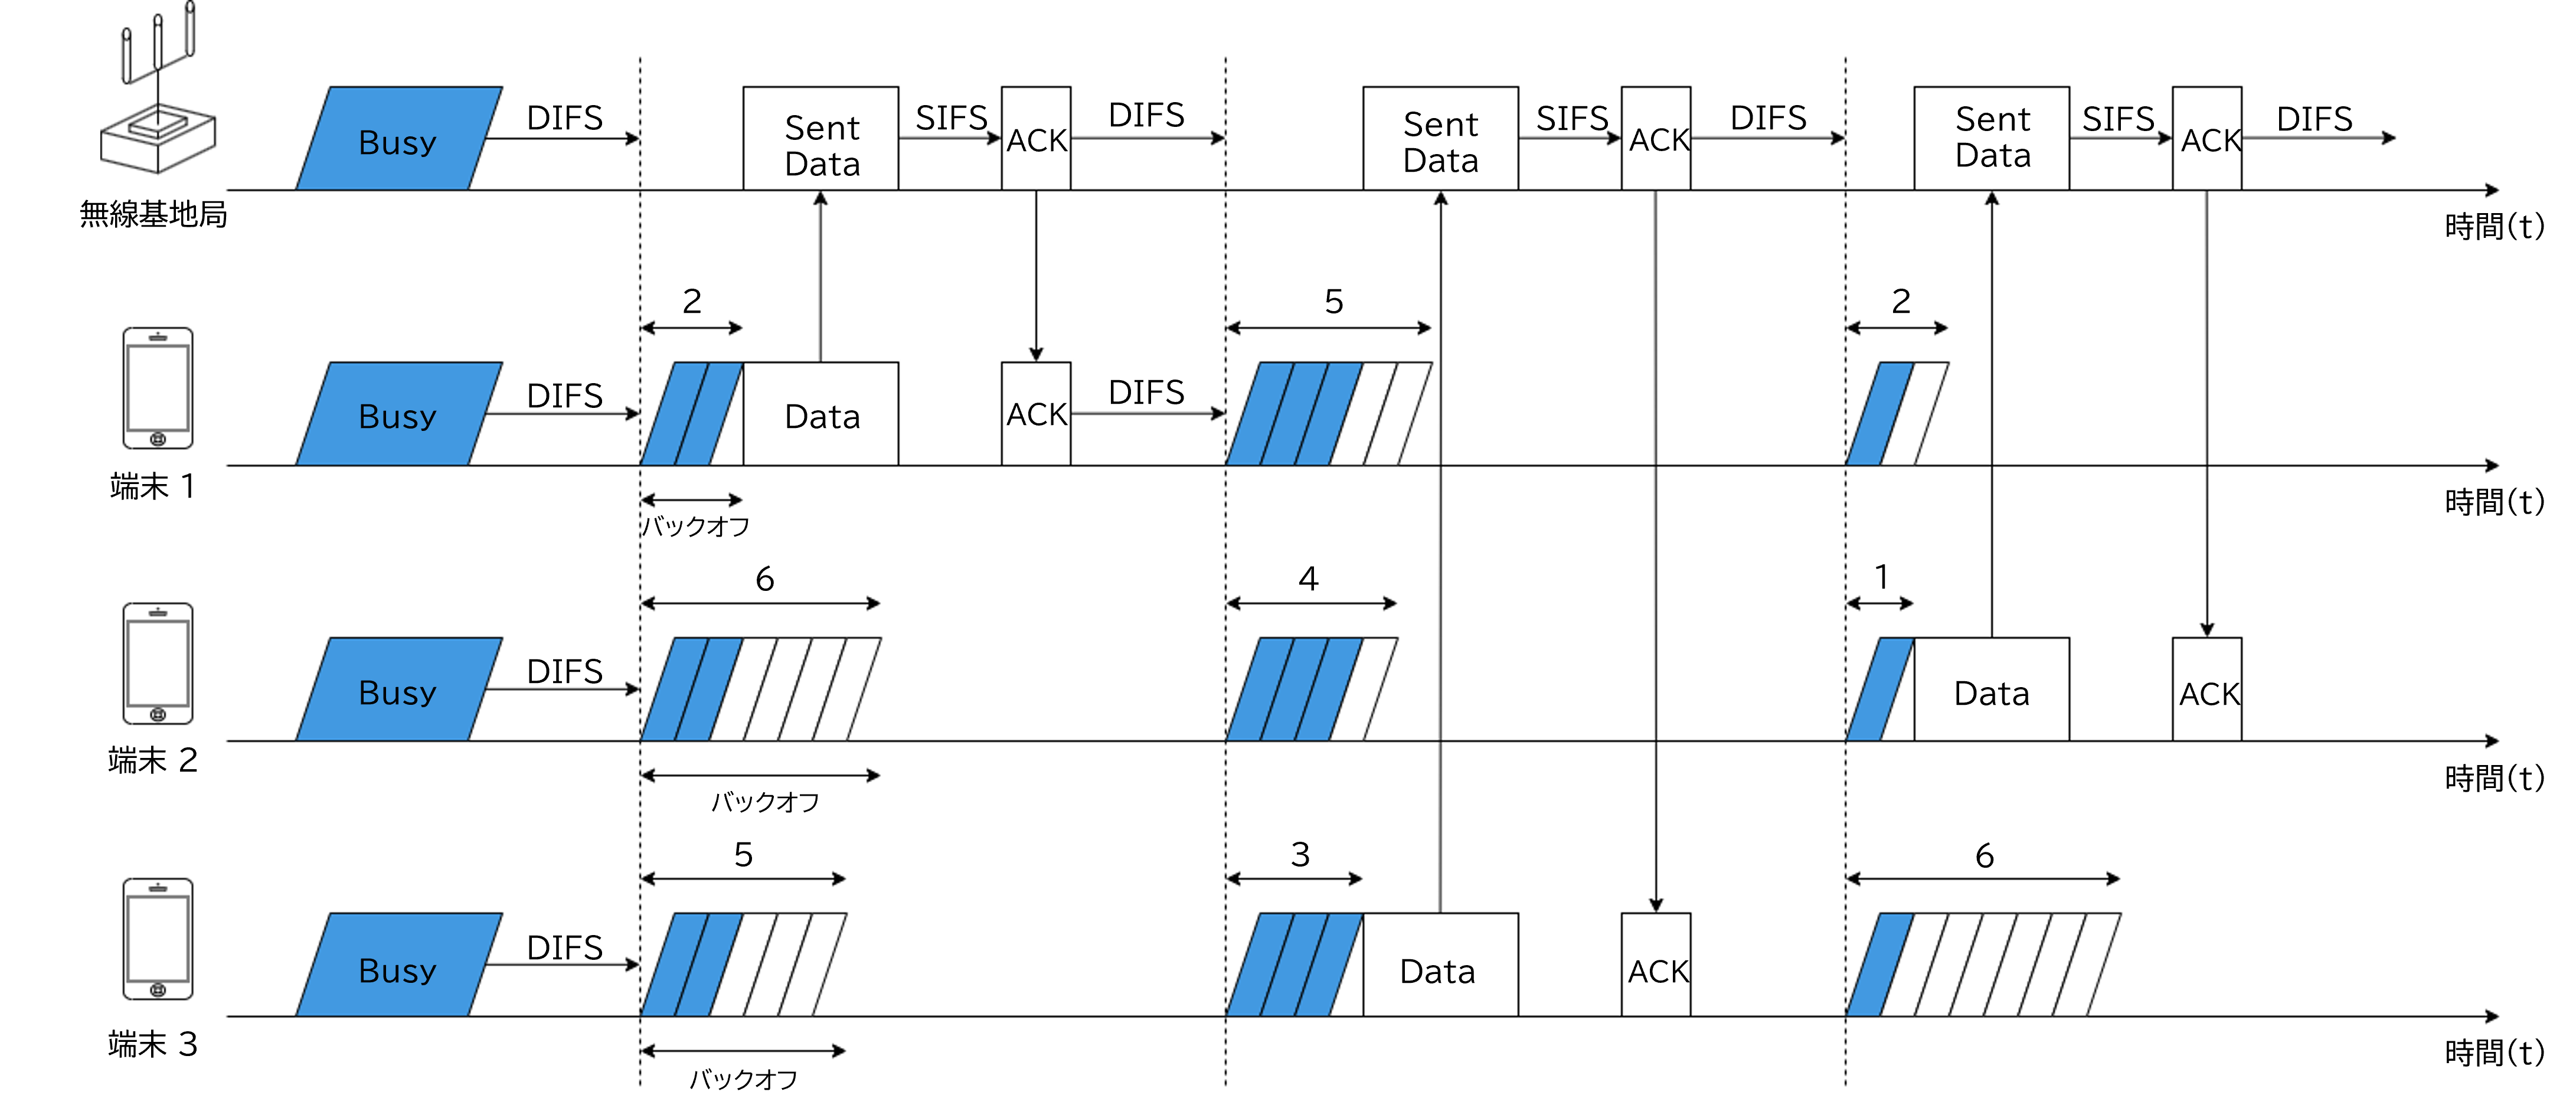
\includegraphics[width=1\textwidth]{./assets/csma-ca-s.png}
    \caption{CSMA/CA成功例}
    \label{1a}
  \end{subfigure}


  \begin{subfigure}{\textwidth}
    \centering
    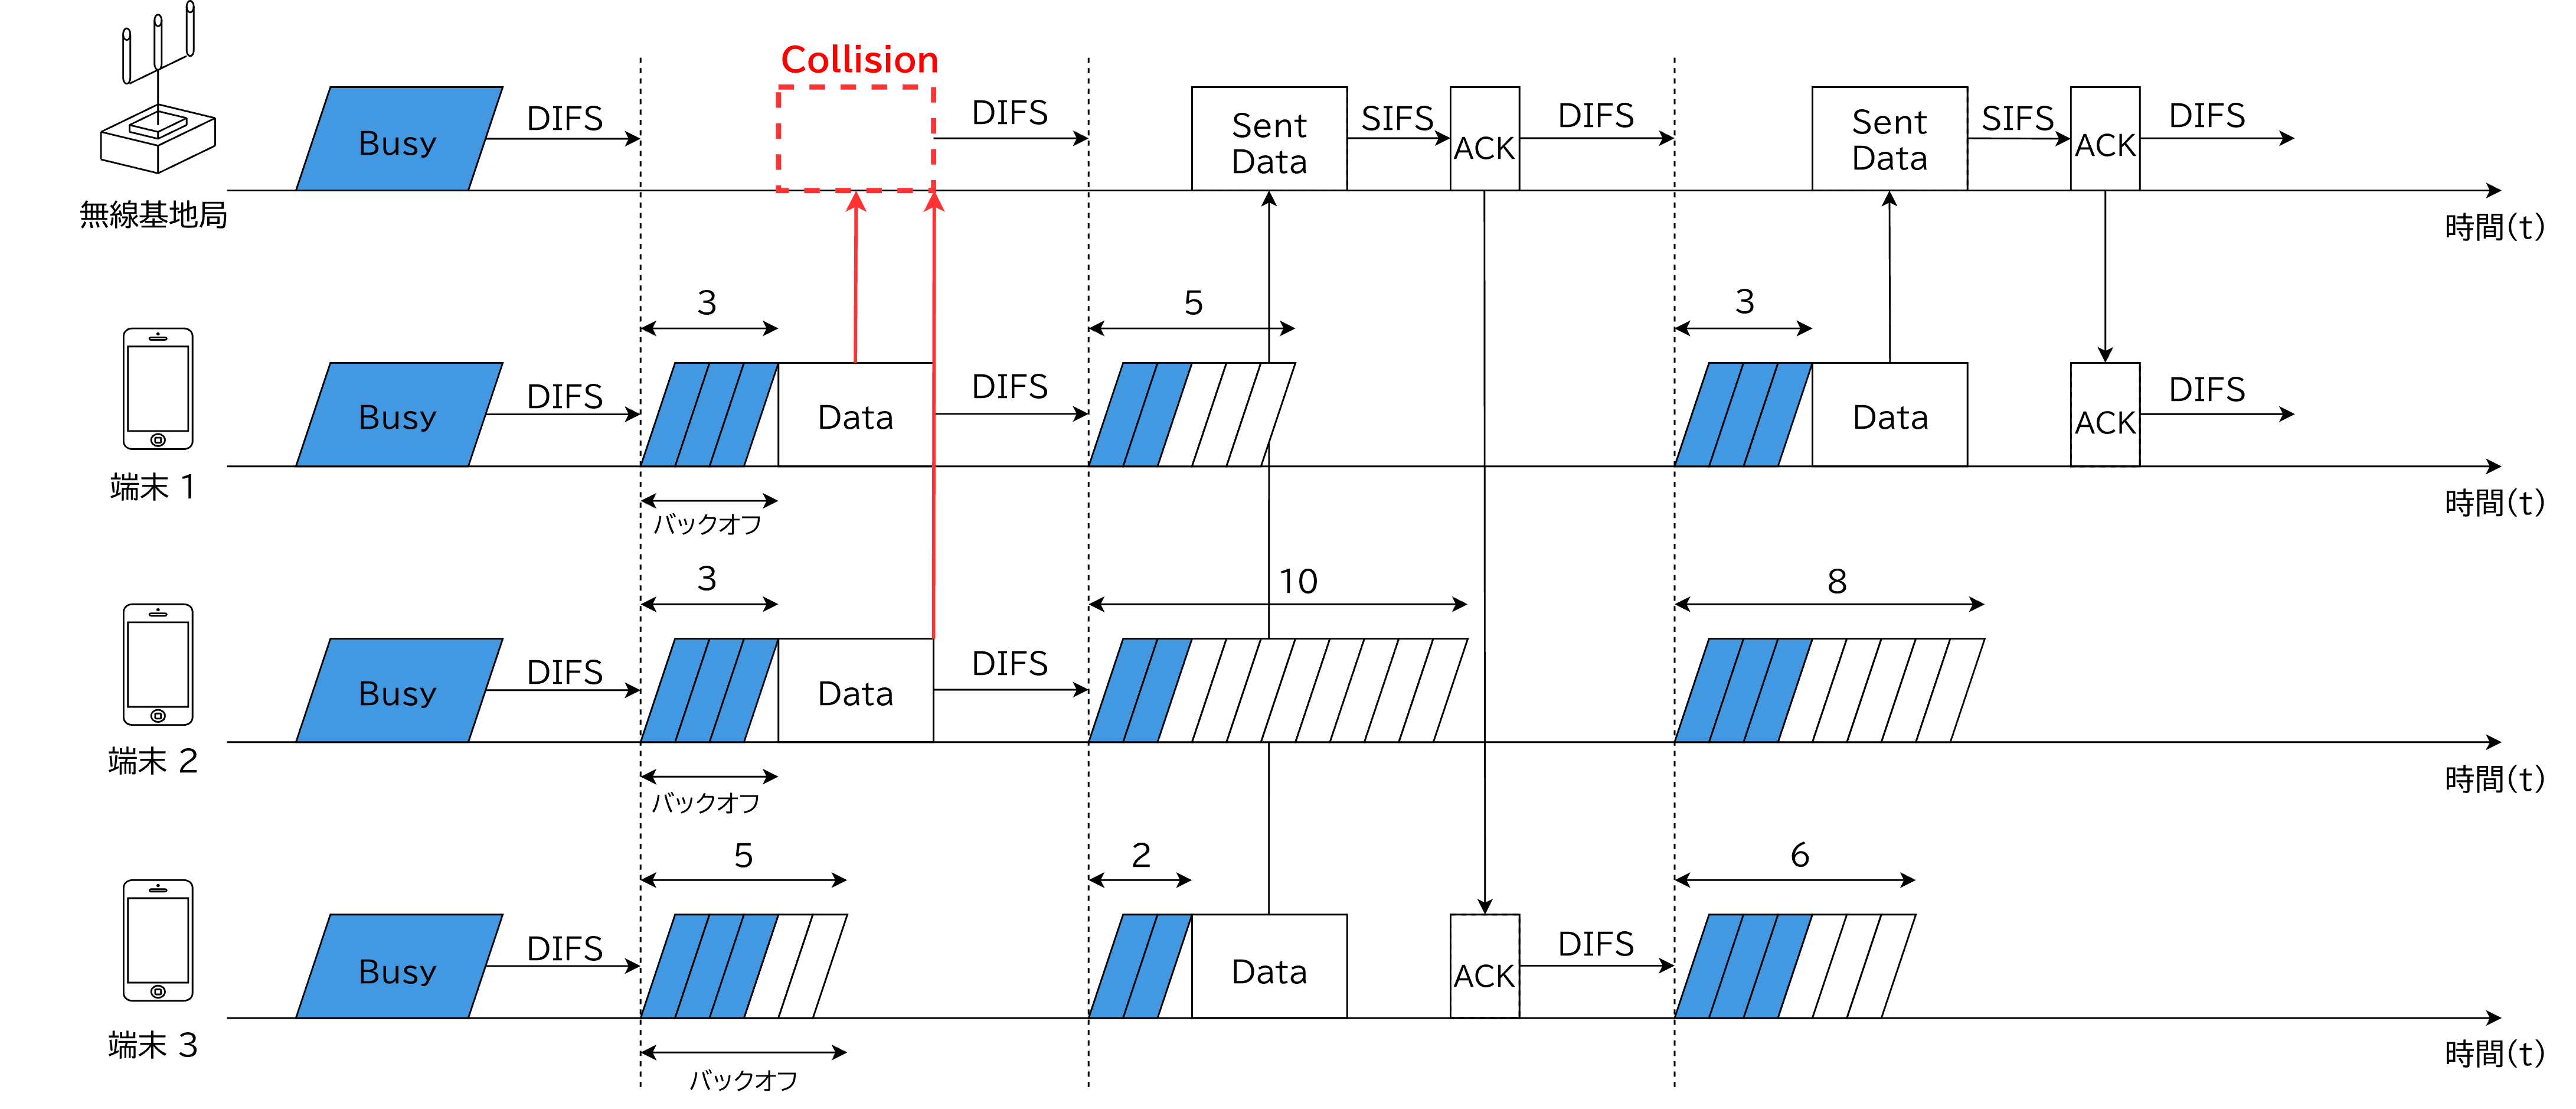
\includegraphics[width=1\textwidth]{./assets/csma-ca-f.png}
    \caption{CSMA/CA衝突例}
    \label{1b}
  \end{subfigure}


  \caption{CSMA/CAの概要}
  \label{CSMA/CA}
\end{figure}


\begin{figure}[H]
  \centering
  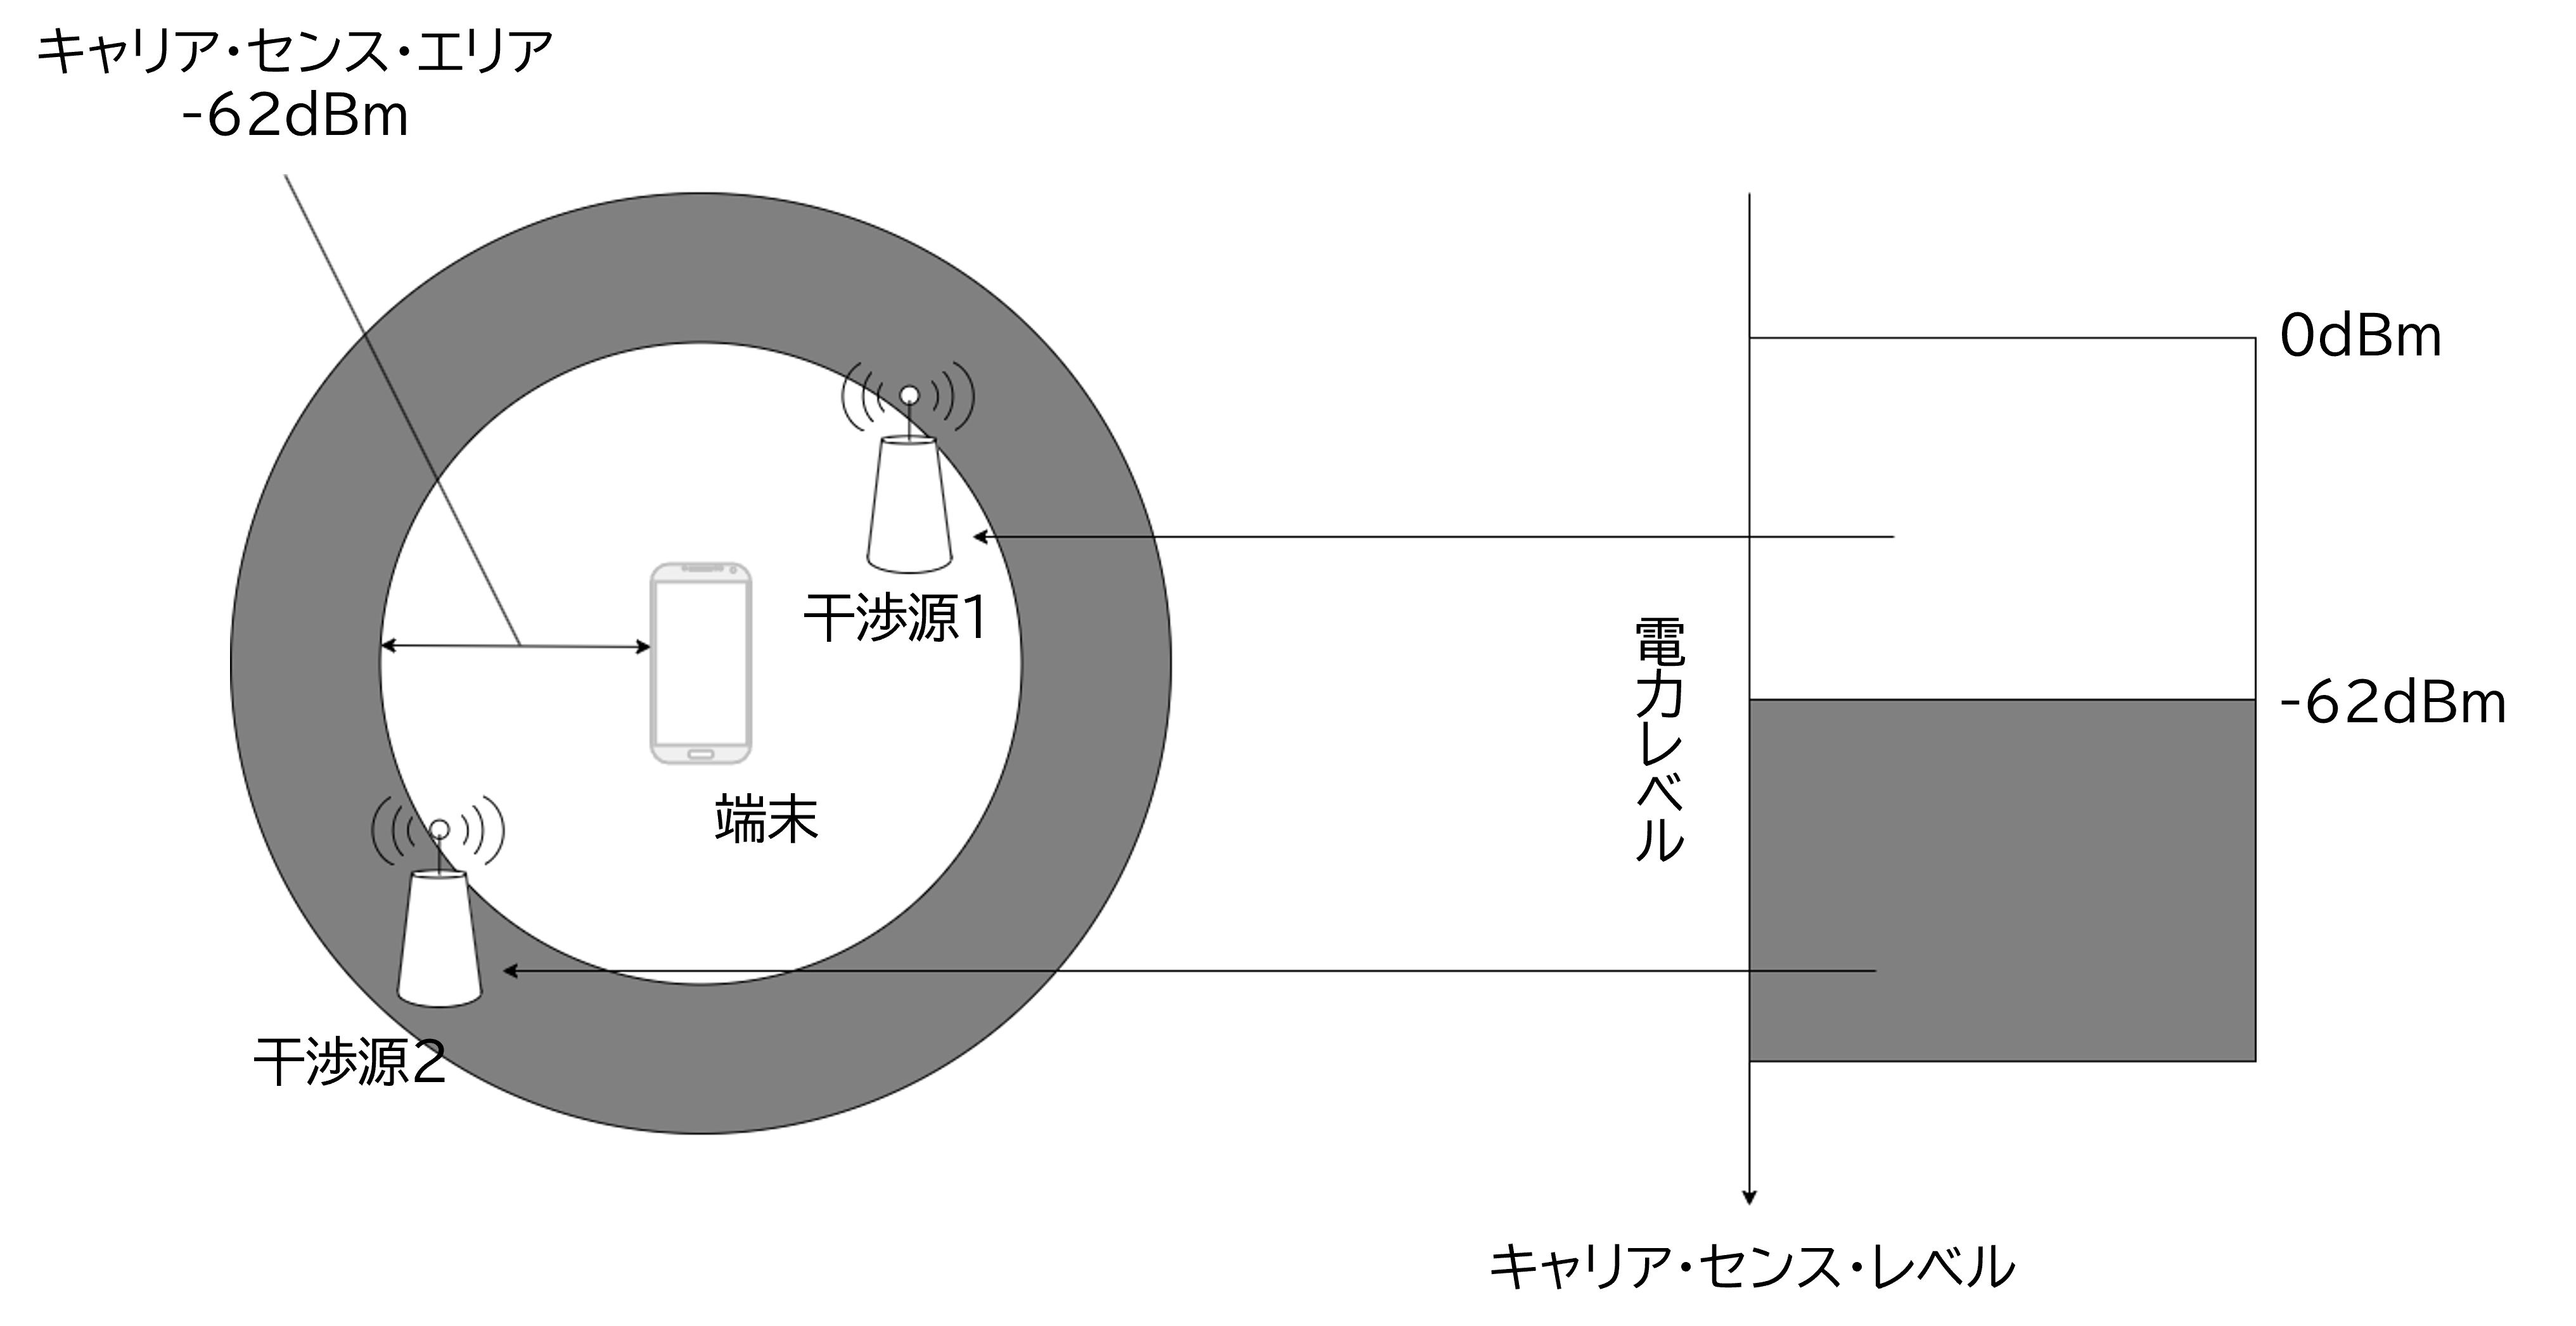
\includegraphics[width=\textwidth]{./assets/CS_level.png}
  \caption{キャリアセンスレベル\cite{midori}}
  \label{fig:CS_level}
\end{figure}


\subsubsection{2進数バックオフ方式}

無線LANシステムでは2進数バックオフ方式を採用している.バックオフ制御では,チャネルが一定時間Idleであれば,フレームを送信しようとする無線局は,規定のContention Window(CW)範囲内で乱数を発生させ,その乱数値を元にしたランダム時間(バックオフ時間)が決められる.概要を図\ref{binary-backoff}に示す.


CWサイズは,最小値($\mathrm{CW_{min}}$)を15とし,最大値の上限($\mathrm{CW_{max}}$)を1023スロットとして衝突回数の増加に従いスロット数$s$は


\begin{align}
  \mathrm{CW}_{\max} &= 2^{4 + n} - 1
\end{align}

\begin{align}
  s &= \mathrm{randint}(0, \, \min(\mathrm{CW}_{\max}, \, 1023))
  \label{slot}
\end{align}

で求められる.ここで,$n$は再送回数,$\mathrm{CW}_{\max}$はCWサイズの最大値である.

再送を繰り返し,$\mathrm{CW_{max}}$に達したときはあらかじめパラメータで決められた最大再送回数M回となるまでCWサイズは$\mathrm{CW_{max}}$のままで再送を繰り返し,
M回を超えると送信失敗となり,フレームが破棄される.

衝突が発生するたびにCWサイズの最大値は2倍に増加するため,再送回数が増えるほどバックオフ時間が長くなることで他端末と同じCWサイズを生成することがなくなり,衝突確率を低減することができる.一方で,2進数バックオフ方式ではCWサイズの増加がオーバーヘッドを引き起こし,スループットの低下につながる.


本シミュレータでは,端末単位でスロット数と再送回数$n$を保持することで,各端末が送信を試みる際の待機時間を動的に設定する処理を実装した.

\begin{figure}[H]
  \centering
  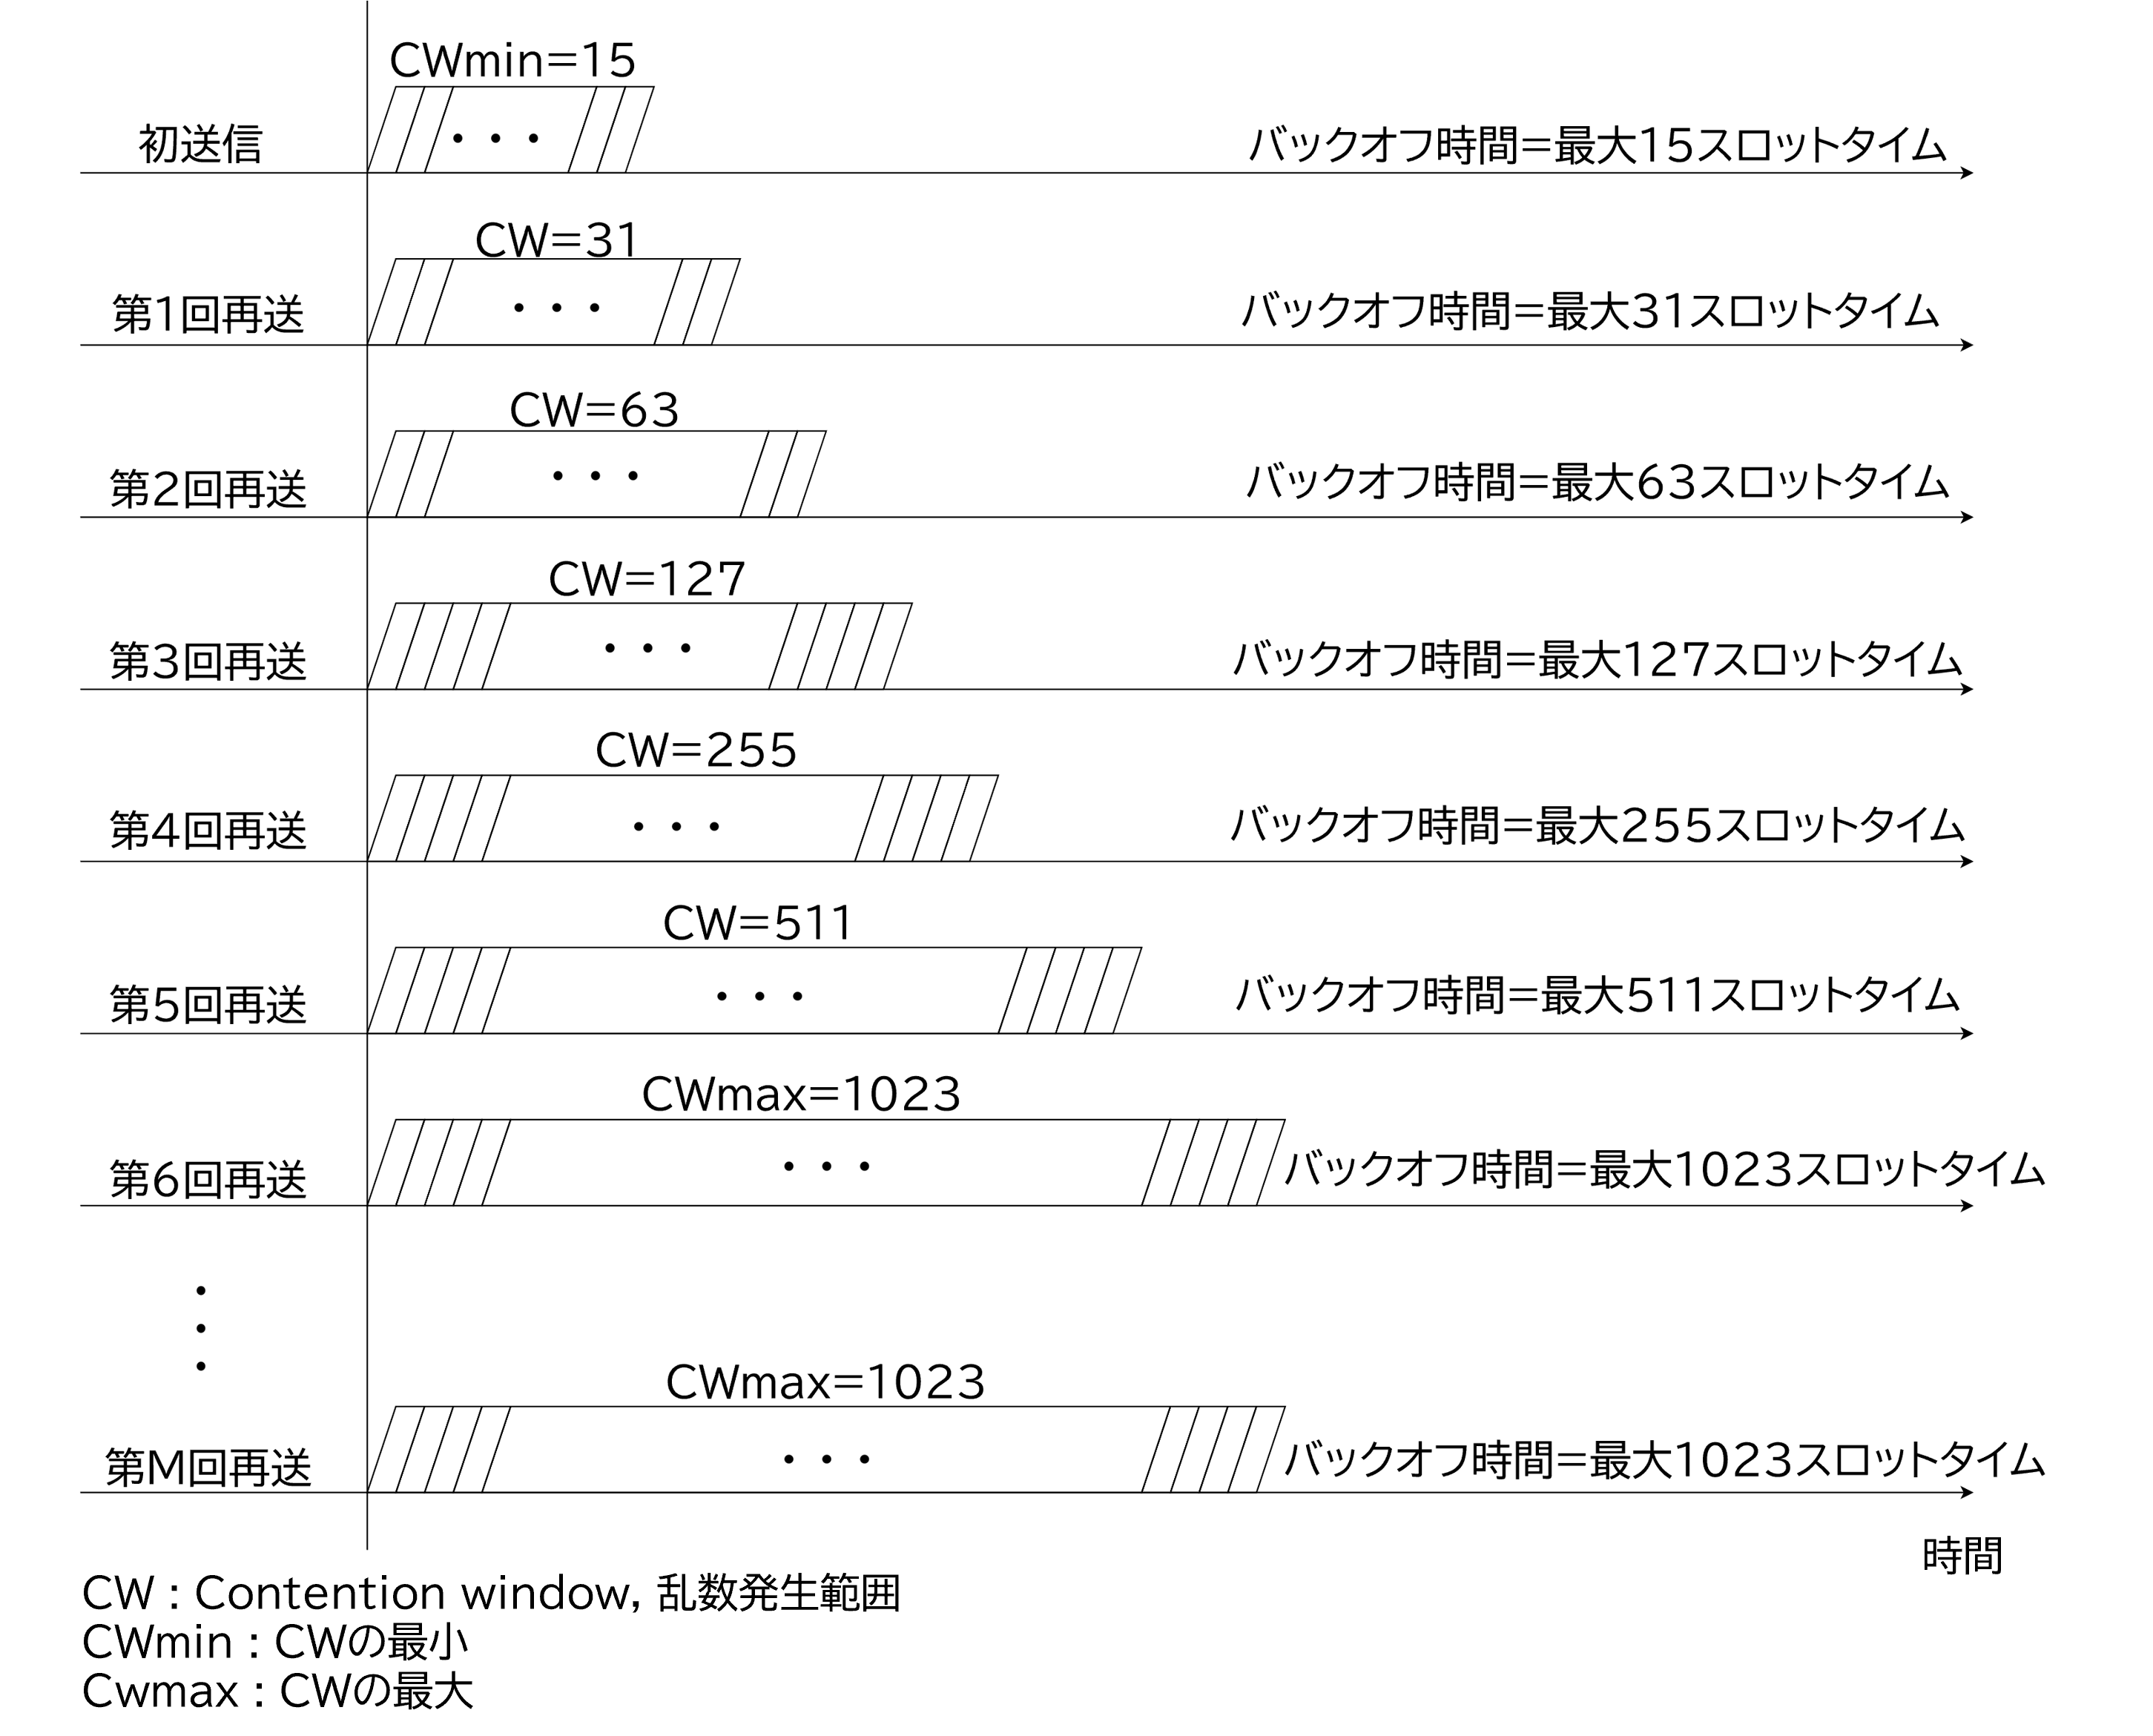
\includegraphics[width=\textwidth]{./assets/CW_.png}
  \caption{2進数バックオフ方式}
  \label{binary-backoff}
\end{figure}


\clearpage
\subsubsection{IFSによる優先制御}

フレーム間にはIFS(Inter Frame Space)と呼ばれる待機時間が設定されている.IFSの長さは6種類存在し,代表的なものにDIFS(Distributed Inter Frame Space)とSIFS(Short Inter Frame Space)がある.これらは,フレームの優先順位に基づいてどのIFSを選択するかが決定される.

DIFSはデータフレーム送信時に適用されるIFSであり,端末は送信開始前にDIFS時間($34\mathrm{\mu s}$)待機してからデータフレームを送信する.
一方,ACKフレームのように失敗すると再送制御が必要となる優先度の高い制御フレームは,DIFS時間待つと他端末のデータフレームと競合する可能性があるため,より短いSIFS時間($16\mathrm{\mu s}$)を用いることで優先的に送信するように設定されている.

\begin{figure}[H]
  \centering
  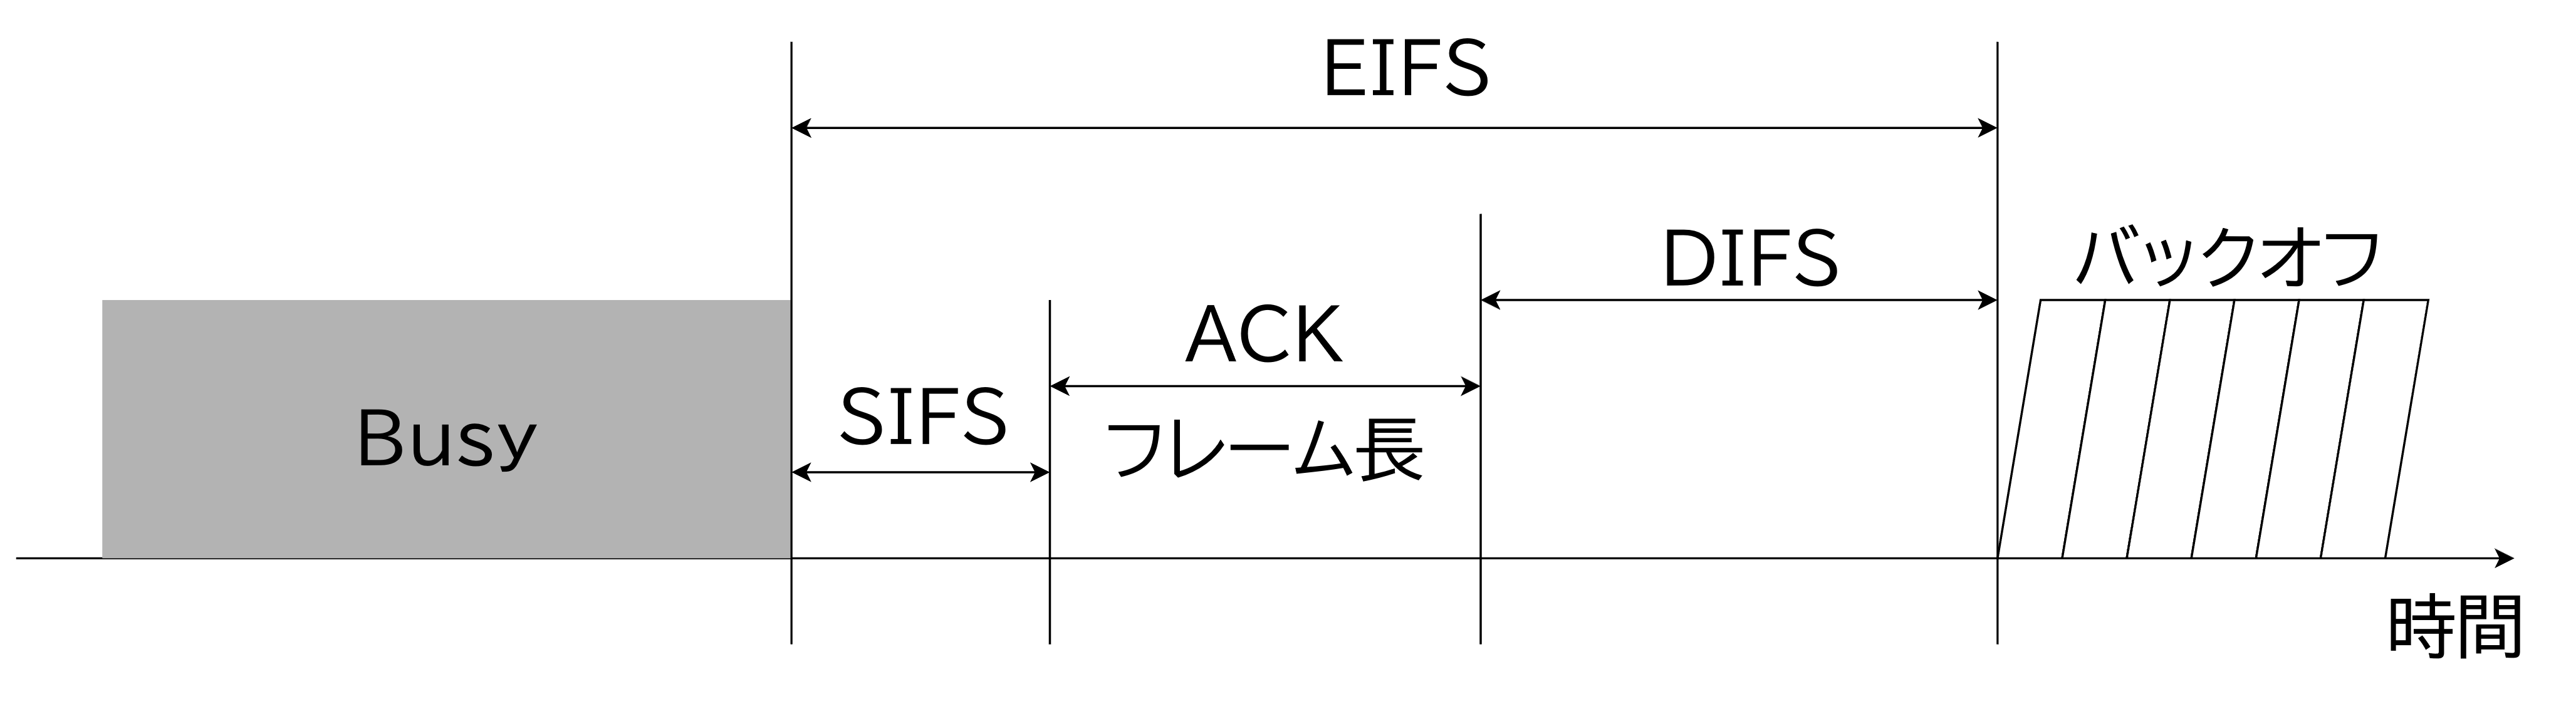
\includegraphics[width=0.8\textwidth]{./assets/EIFS.png}
  \caption{EIFSの送出信号間の間隔}
  \label{eifs}
\end{figure}


\subsubsection{フレーム構成モデル化}

本研究では,MAC層に着目した無線LAN通信の挙動を評価するため,UDP(User Datagram Protocol)レベルのフレーム構成をモデル化し,図\ref{packet}にその構成図を示す.

無線LANフレームにはPLCP(Physical Layer Convergence Protocol)プリアンブルやMACヘッダー,FCS(Frame Check Sequence)に加え,LLC(Logical Link Control)ヘッダやIPヘッダなども含まれるが,シミュレーションの都合上省略し,モデル化した.

無線LAN通信では,データ送受信時にPLCP(Physical Layer Convergence Protocol)プリアンブルやMACヘッダ,FCS(Frame Check Sequence)などの制御情報のオーバーヘッドに加え,ACKフレームの送信やCSMA/CA特有のDIFS・SIFSなどのフレーム間隔,バックオフ動作も必要となる.

\begin{figure}[H]
  \centering
  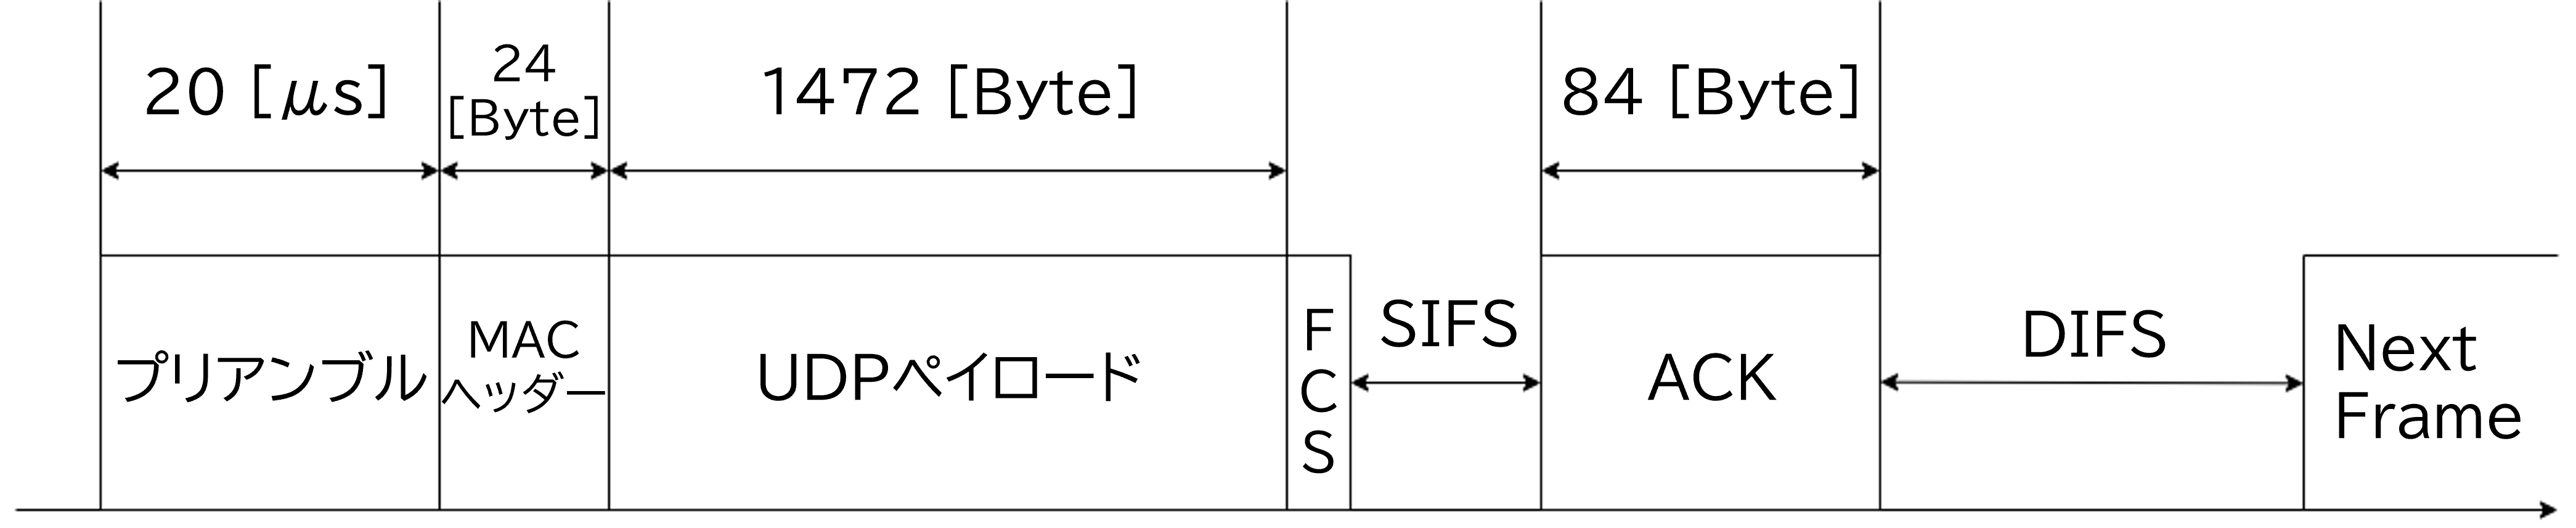
\includegraphics[width=1\columnwidth]{./assets/packet.png}
  \caption{フレーム構成図}
  \label{packet}
\end{figure}


\clearpage
\subsubsection{MCS Index}
MCS(Modulation and Coding Scheme) Indexは,変調方式と符号化率の組み合わせを示す指標である.IEEE 802.11 規格では,環境に応じて適応的に変更可能な MCS インデックスが定義されており,これにより通信の信頼性と伝送速度の最適化を図ることが可能である.MCS インデックスは 0 から最大値(規格により異なる)まで定義され,値が大きくなるほど高次の変調方式(QPSK,16QAM,64QAM 等)と高符号化率が採用される.これにより理論上の伝送速度は向上するが,必要とされる信号対雑音比(SNR : Signal-Noise Ratio)も増加する.実際の通信では,受信電力レベルや干渉状況に基づいて適切な MCS インデックスを選択することで,安定した通信品質を確保することが重要となる.

表\ref{table:mcs_11abg_rssi}にMCS INDEXの例を示す.
本シミュレータでは,実際の通信環境をより現実的に模擬するために同様のMCSインデックスを定義し,RSSI (Received Signal Strength Indicator)から決定された伝送レートを受け取る.\\


\begin{table}[H]
  \centering
  \caption{IEEE 802.11a/gのMCSインデックスと要求RSSI}
  \label{table:mcs_11abg_rssi}
  \begin{tabular}{c|c|c|c|c|c|c}
      \hline
      \multicolumn{4}{c|}{IEEE 802.11a} & \multicolumn{3}{c}{IEEE 802.11g} \\
      \hline
      変調方式 & 符号化率 & レート (Mbps) & RSSI (dBm) & 変調方式 & レート (Mbps) & RSSI (dBm) \\
      \hline
      BPSK & 1/2 & 6 & -82 & DBPSK/CCK & 1 & -94 \\
      BPSK & 3/4 & 9 & -81 & DQPSK/CCK & 2 & -91 \\
      QPSK & 1/2 & 12 & -79 & CCK & 5.5 & -89 \\
      QPSK & 3/4 & 18 & -77 & CCK & 11 & -85 \\
      16-QAM & 1/2 & 24 & -74 & BPSK-OFDM & 6 & -82 \\
      16-QAM & 3/4 & 36 & -70 & QPSK-OFDM & 12 & -79 \\
      64-QAM & 2/3 & 48 & -66 & 16QAM-OFDM & 24 & -74 \\
      64-QAM & 3/4 & 54 & -65 & 64QAM-OFDM & 54 & -65 \\
      \hline
  \end{tabular}
\end{table}


\clearpage
\subsubsection{マルチレート(複数の伝送レート)のサポート}

802.11無線LANでは,無線局が複数の伝送レートをサポートすることが可能.例として802.11bでは,11, 5.5, 2, 1\, Mbpsの4つ,802.11aでは54, 48, 36, 24, 18, 12, 9, 6\, Mbpsの8つ(54, 48, 36, 18, 9Mbpsはオプション)の伝送レートが規定されている.

伝送レートが低いほど長距離の通信を行うことができるので,図\ref{multirate}に示すように,基地局は自局近傍の端末とは高い伝送レートで通信を行い,遠くの端末とは低いレートに切り替えて通信を行うと,広いエリアで効率的に通信を行うことができる.なお,適切な伝送レートを選択するアルゴリズムについては,802.11で規定されていないため,無線LANベンダが独自に実装する必要がある.


\begin{figure}[H]
  \centering
  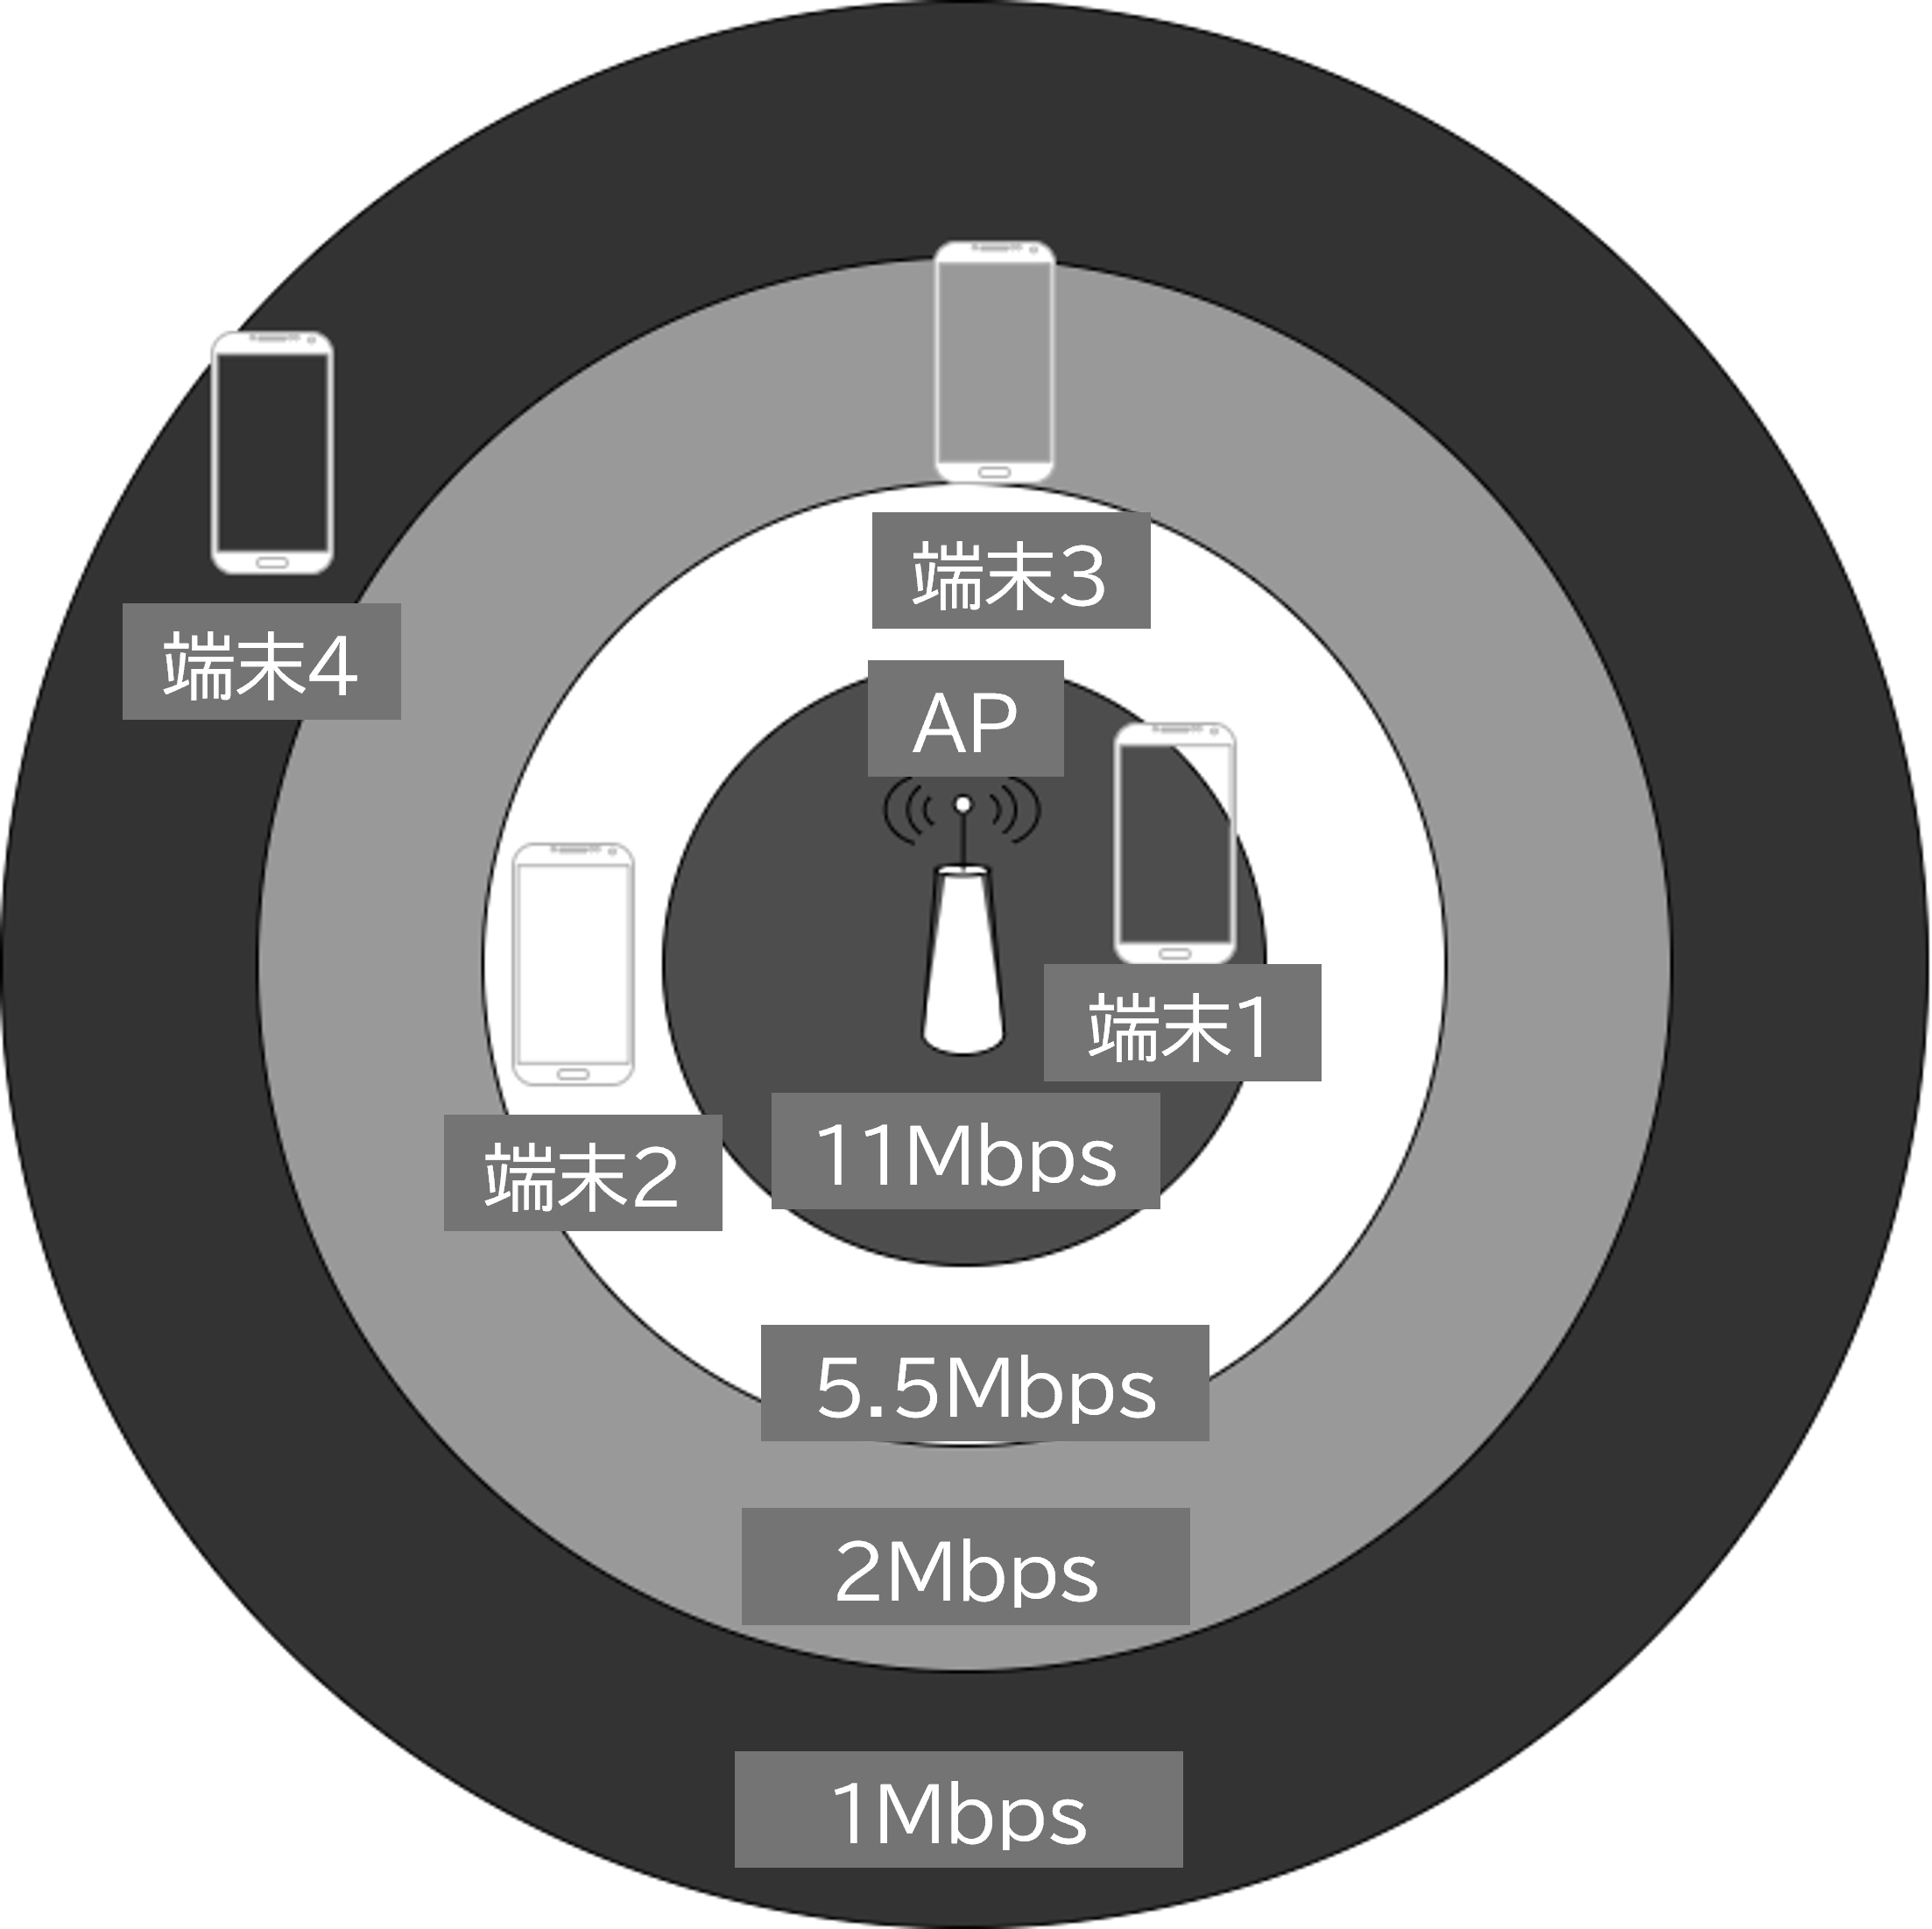
\includegraphics[width=0.8\textwidth]{./assets/multilate.png}
  \caption{複数の伝送速度が可能なマルチレート通信環境(802.11bの例)}
  \label{multirate}
\end{figure}

\clearpage

\subsection{課題}
本研究では電波伝搬特性を考慮した物理層シミュレータと連携して,MAC層の動作を評価するクロスレイヤシミュレータを提案する.本シミュレータでは物理層シミュレータから受信感度に応じてチャネルの伝送レートを受け取り,その値に基づいてプロトコルの評価を行う.

しかし,クロスレイヤ評価を行うためには様々な課題がある.図\ref{fig:problem}に課題の概要を示す.まず,現実環境に即したクロスレイヤ評価方法として実機実験によるフィールド評価がある.実機実験は無線デバイス等で実際に通信するため,物理層からアプリケーション層までを考慮することができるため,現実環境による評価ができるメリットがある.しかし,実機による実験は時間的制約,人的リソースおよび無線デバイスの開発費用など実験に莫大な費用と手間がかかるのが大きな問題である.また,伝搬実験のみを実際に行う場合でも,フィールド試験を行うには多くの時間と労力が必要である.さらに,上位層との連携評価が難しいことも課題として残っている.以上のことから実機実験を伴わない計算機上での評価方法の確立が今後必要となっている\cite{book2}.

\begin{figure}[H]
  \centering
  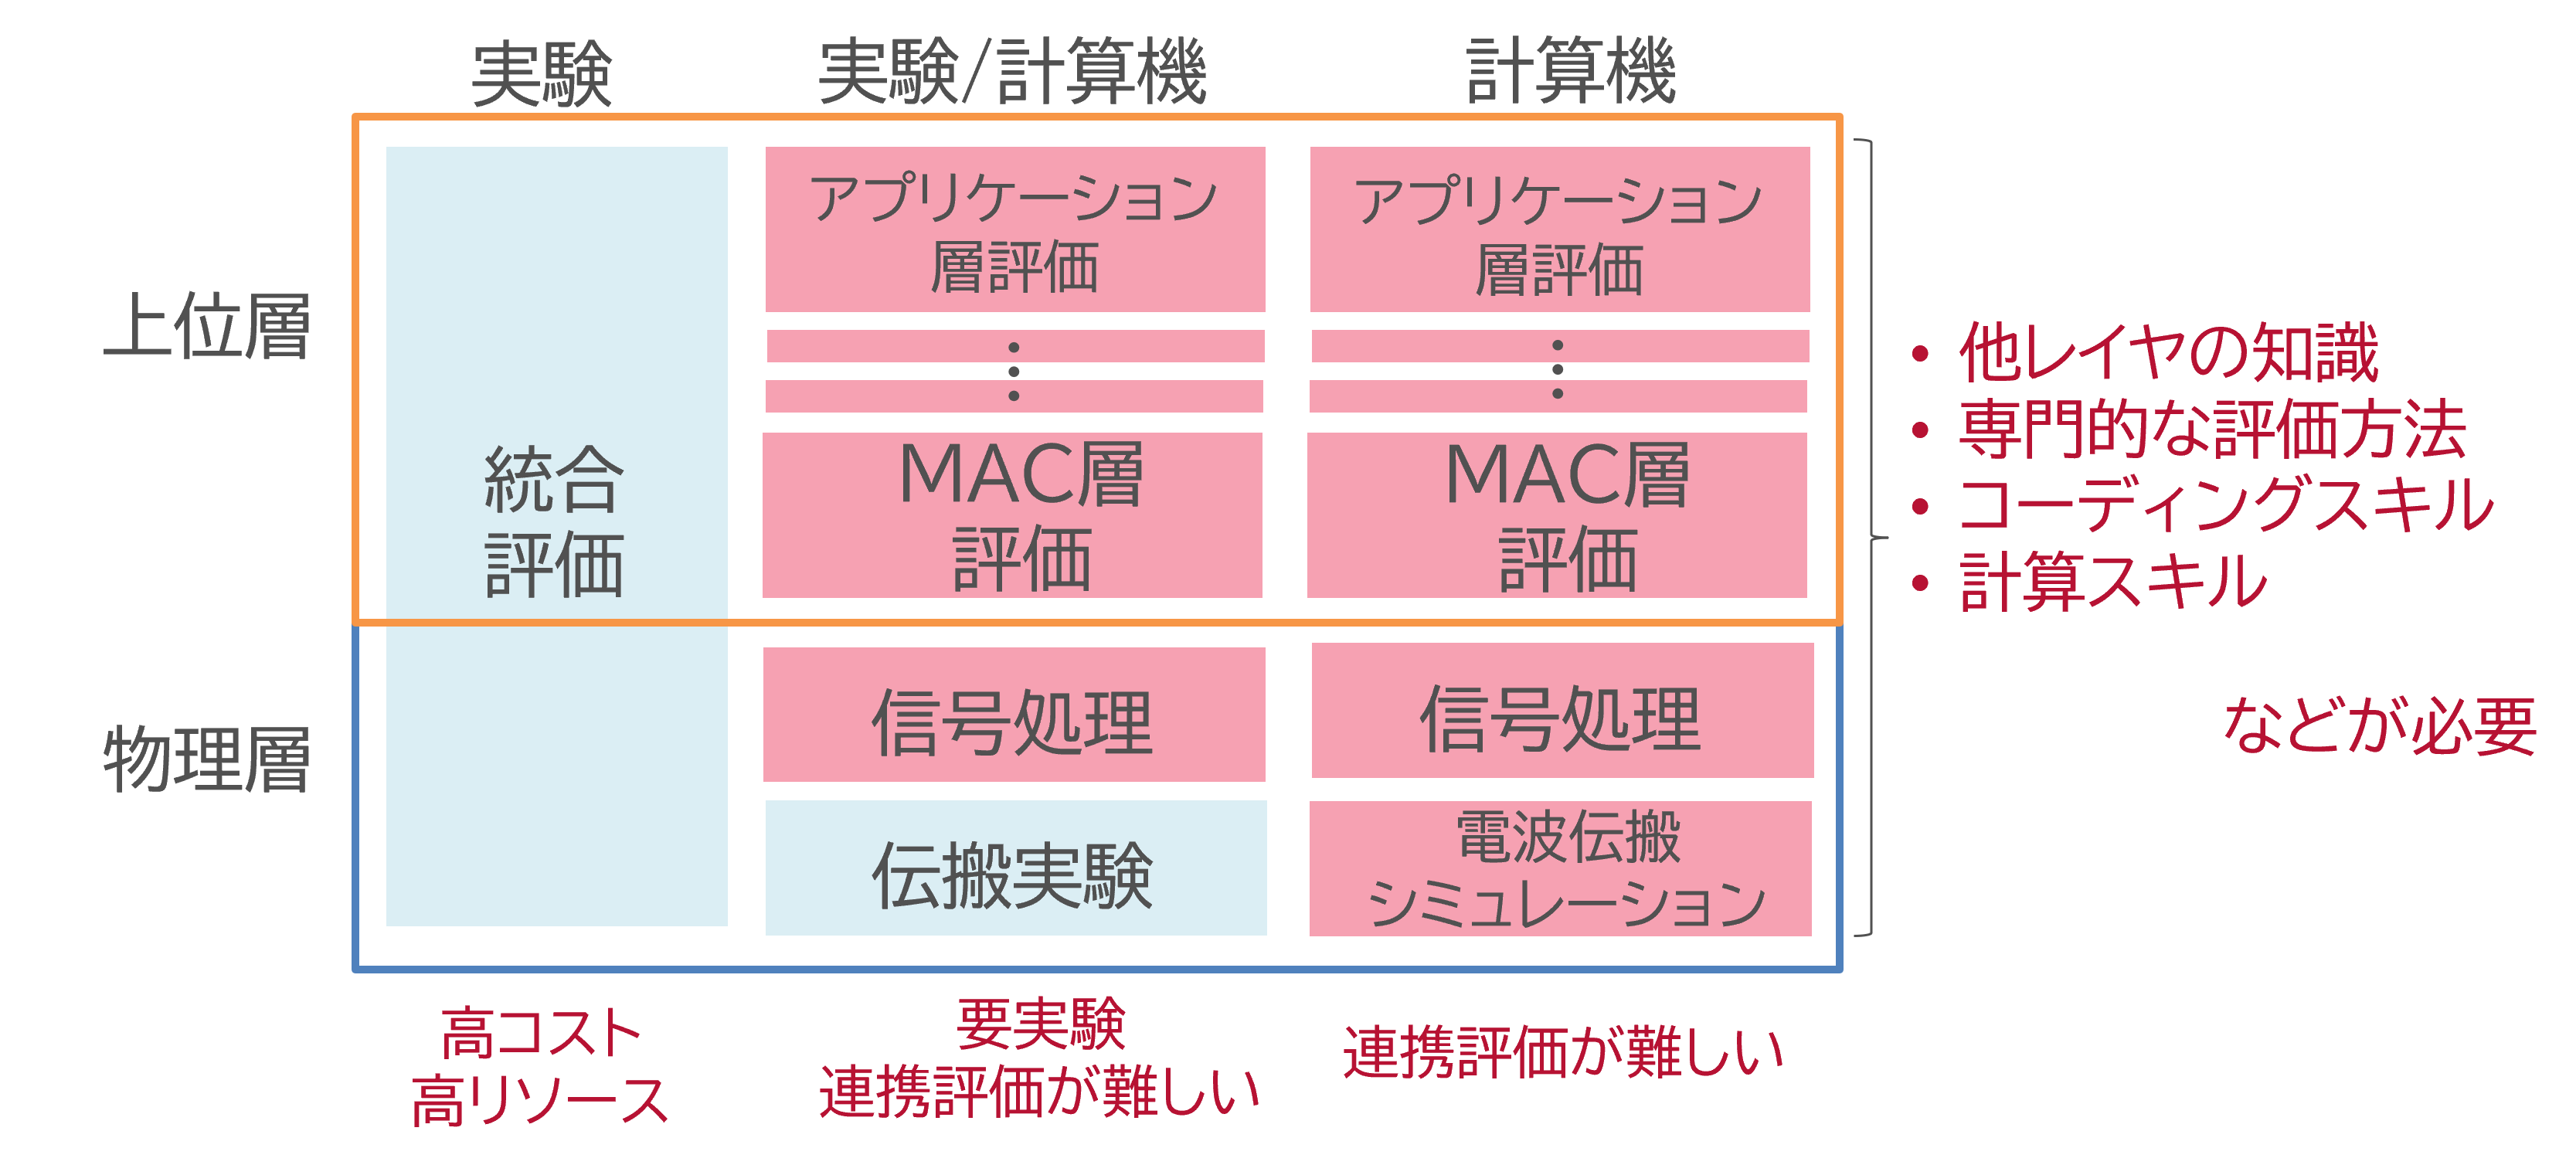
\includegraphics[width=\textwidth]{./assets/課題.png}
  \caption{クロスレイヤシミュレータの課題}
  \label{fig:problem}
\end{figure}



% ******************************************************
% 提案モデル
% ******************************************************
\clearpage
\section{提案モデル}

\subsection{実装}

本研究では,CSMA/CA方式を用いた無線LANを再現するために,Pythonを用いてシミュレータを作成した.シミュレータには,各端末を管理する端末クラスを導入し,端末ごとのCWサイズや再送回数の管理,バックオフ時間を決定するためのスロット数の管理,再送処理などの機能を実装している.

また,シミュレータ本体は標準ライブラリである\texttt{random}のみに依存するように設計した.これにより,バージョン差異による影響を受けにくい後方互換性のあるシミュレータを実現した.


\subsection{動作環境}

表\ref{tab:env}に本シミュレータの動作環境と使用ライブラリを示す.



\begin{table}[h]
  \centering
  \caption{動作環境と使用ライブラリ}
  \label{tab:env}
  \begin{tabular}{l|l|l}
      \hline
      カテゴリ & 項目 & バージョン \\ \hline
      Language           & Python        & 3.10.12 \\ 
      &               & 3.11.11 \\ \hline
      ライブラリ       & random         & \\ \hline
      OS               & Ubuntu        & 22.04 LTS \\ 
                       & Debian        & 12 \\ \hline
  \end{tabular}
\end{table}


\clearpage
\subsection{フローチャート}
図\ref{flowchart}に本シミュレータのフローチャートを示す.


\begin{figure}[H]
  \centering
  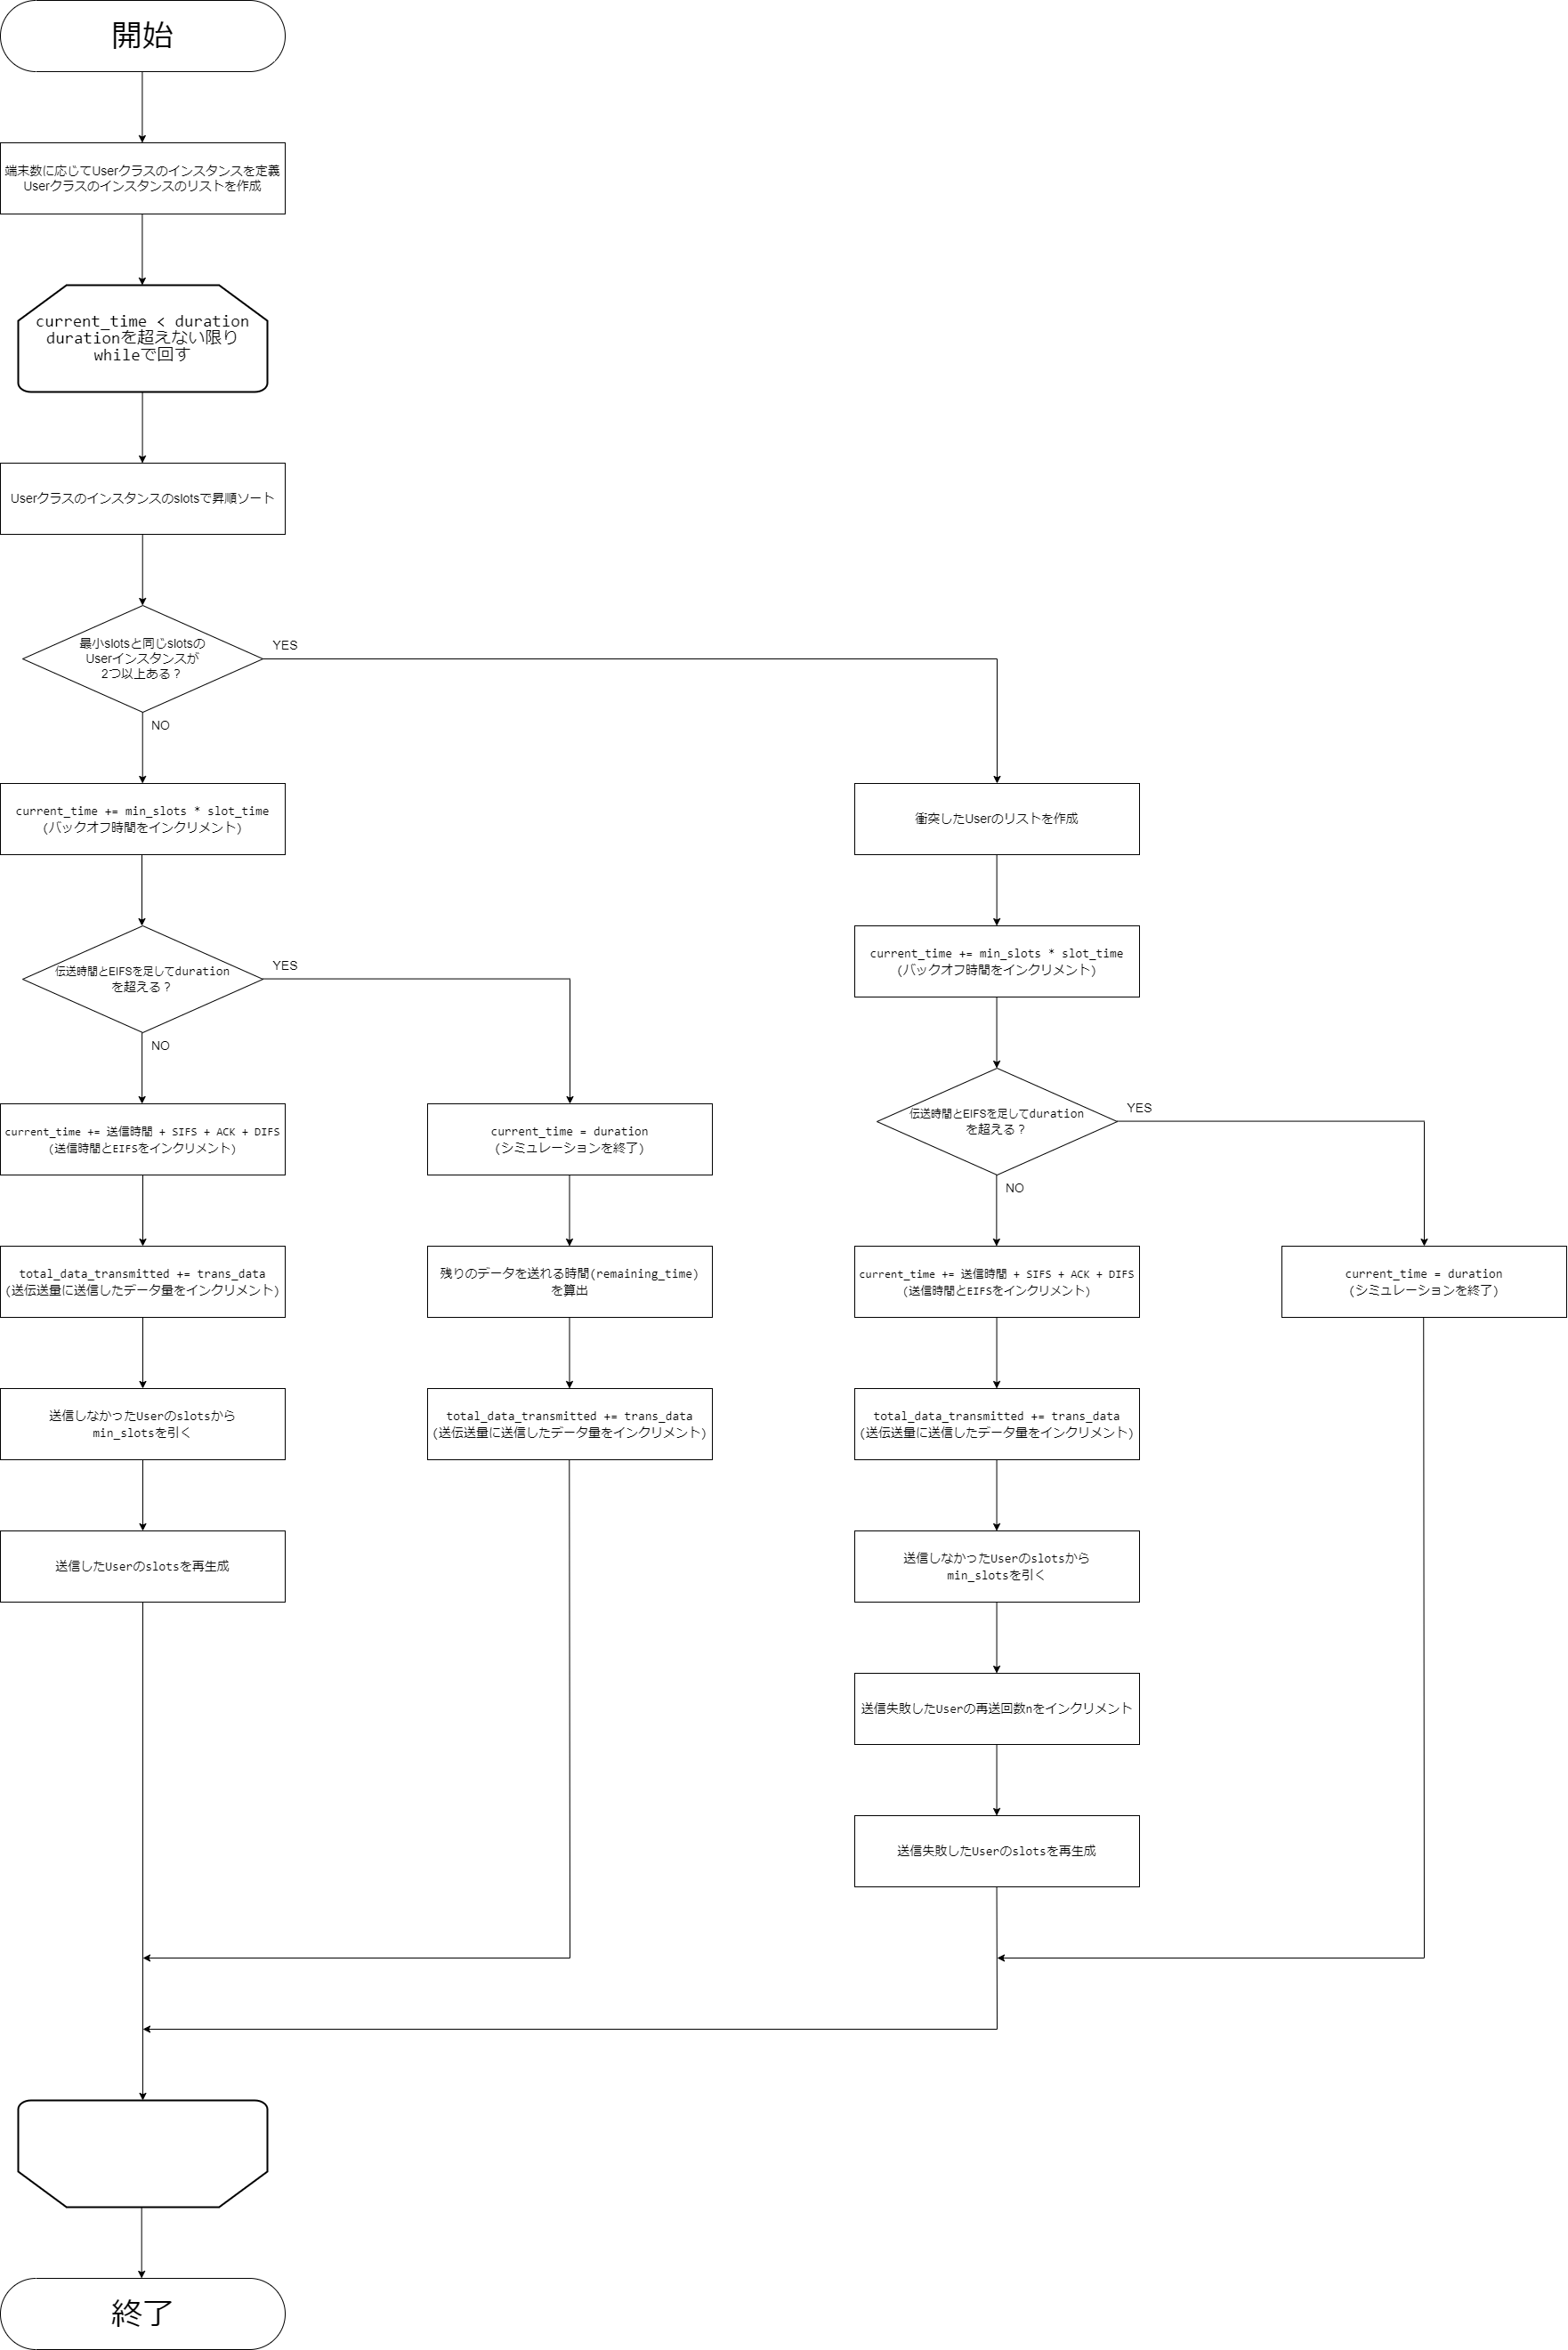
\includegraphics[width=0.9\textwidth]{./assets/flowchart.drawio.png}
  \caption{フローチャート}
  \label{flowchart}
\end{figure}



\subsection{\texttt{User}クラスの設計}
本研究のシミュレータ実装では,各端末を\texttt{User}クラスとして定義し,端末ごとのCWや再送回数などを管理している.表\ref{tab:user-class}に主なメンバ変数と役割をまとめる.

各端末を端末クラスのインスタンスとして定義することで,個別のバックオフ制御を実現している.新しいプロトコルや機能を追加する際にも,\texttt{User}クラスを継承することで容易に拡張できるように設計した.

\begin{table}[H]
  \centering
  \caption{Userクラスのメンバ変数とメソッドの一覧}
  \label{tab:user-class}
  \begin{tabularx}{0.5\textwidth}{l|X}
    \hline
    % \textbf{名称} & \textbf{説明} \\
    名称 & 概要 \\
    \hline
    \multicolumn{2}{l}{メンバ変数} \\
    \hline
    \texttt{id} & 端末を識別するためのID\\
    \texttt{num\_re\_trans} & 再送回数\\
    \texttt{slots} & スロット数\\
    \texttt{num\_transmitted} & 送信成功回数\\
    \texttt{data\_transmitted} & 送信したデータ量 \, [bit]\\
    \hline
    \multicolumn{2}{l}{主なメソッド} \\
    \hline
    \texttt{calc\_slots()} &(\ref{slot})式に従い\texttt{slots}を決定\\
    \texttt{re\_transmit()} & 再送処理\\
    \texttt{reset\_slots()} & 新たに\texttt{slots}を割り当てる\\
    \hline
  \end{tabularx}
\end{table}

\subsection{シミュレーション条件例}
表\ref{tab:sim-param}に,本研究で用いたシミュレーション条件を示す.
モードを選択することでそれぞれの無線LAN規格(IEEE 802.11a/b/g)に対応できるように設計した.

また,各モードに対応するパラメータはシミュレータプログラム内の辞書型で管理されているため,新しい規格やパラメータを追加する際には辞書型に追加することで容易に対応できるように設計した.

\begin{table}[H]
  \centering
  \caption{シミュレーション条件の例}
  \label{tab:sim-param}
  \begin{tabular}{c|@{\hspace{1.8em}}l}
    \hline
    パラメータ & 値・例 \\
    \hline
    シミュレーション時間 & 60  \,$\mathrm{s}$\, \\
    モード & \, \,  a \\
    スロット時間 (802.11a) & \, 9  \,$\mathrm{\mu s}$\, \\
    DIFS (802.11a) & 34 \, $\mathrm{\mu s}$\, \\
    SIFS (802.11a) & 16 \, $\mathrm{\mu s}$\, \\
    伝送レート & 24 \, Mbps\, \\
    端末数 & 80 \, 台\, \\
    \hline
  \end{tabular}
\end{table}


\clearpage
\subsection{シミュレーション補助ツール}
同条件でのシミュレーションを繰り返し行うための補助ツールをPythonで作成した.このツールは,シミュレーションのパラメータを設定し,指定回数のシミュレーションを自動で実行することができる.シミュレーション結果はCSVファイルとして出力され,様々なツールで容易に解析を行えるようにした.

threadingやmultiprocessingを用いて並列処理を行うことで,複数のシミュレーションを同時に実行することが可能である.これにより,複数のシミュレーションを同時に実行することで,シミュレーションの実行時間を短縮することができる.

また,tqdmを用いて進捗状況を表示することで,図\ref{tqdm}のようにシミュレーションの進行状況をリアルタイムで確認することができる.

表\ref{tab:env_tool}に本ツールの動作環境と使用ライブラリを示す.

\begin{table}[H]
  \centering
  \caption{動作環境と使用ライブラリ}
  \label{tab:env_tool}
  \begin{tabular}{l|l|l}
      \hline
      カテゴリ & 項目 & バージョン \\ \hline
      Language           & Python        & 3.10.12 \\ 
      &               & 3.11.11 \\ \hline
      ライブラリ       & numpy         & 2.1.3\\ 
                      & pandas    & 2.2.3\\
                      & tqdm      & 4.67.1\\
                      & threading & \\
                      &multiprocessing & \\
                      & queue   & \\\hline
      OS               & Ubuntu        & 22.04 LTS \\ 
                       & Debian        & 12 \\ \hline
  \end{tabular}
\end{table}


\begin{figure}[H]
  \centering
  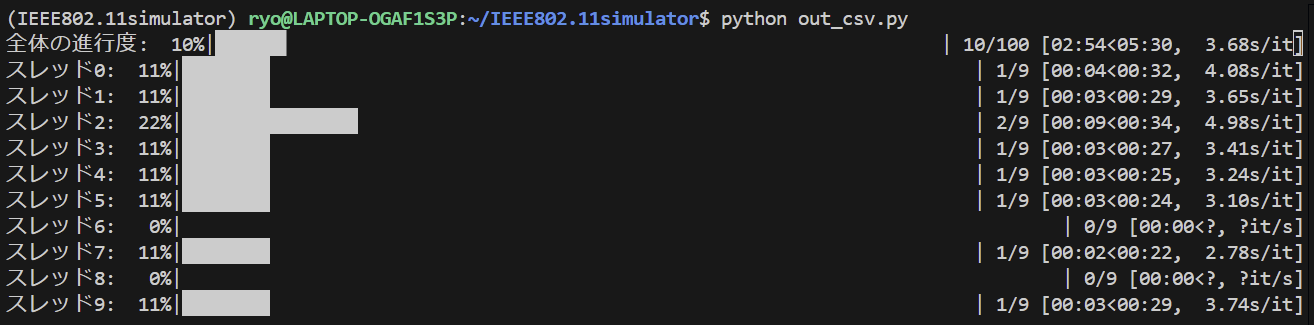
\includegraphics[width=\textwidth]{./assets/tqdm.png}
  \caption{tqdmによる進捗表示}
  \label{tqdm}
\end{figure}


\clearpage
\subsection{提案するクロスレイヤシミュレータの動作}

次に,提案するクロスレイヤシミュレータの動作について説明する.図\ref{fig:cross_simu_flow}に提案するクロスレイヤシミュレータの動作の概要を示す.

ワークフローは以下の順番で実行さる

\begin{itemize}
  \item EEM-RTM上で地形モデル作成
  \item MATLAB上での座標,その他パラメータ設定
  \item EEM-RTM上での伝搬経路解析,パス(伝搬経路)ごとの電力の算出
  \item 解析結果からMATLAB上で合計受信電力を算出
  \item 本CSMA/CAシミュレータを用いたスループット特性の解析
\end{itemize}

ここで,EEM-RTMとは3次元の地形モデリングを行い,そのモデルに基づいた電波伝搬をレイトレース法により高精度に計算が可能なソフトウェアである.また,MATLABは電波伝搬シミュレーション及び解析処理を効率的に行うために採用した.

% 図\ref{fig:cross_simu_flow}に提案するクロスレイヤシミュレータのフローチャートを示す.


\begin{figure}[H]
  \centering
  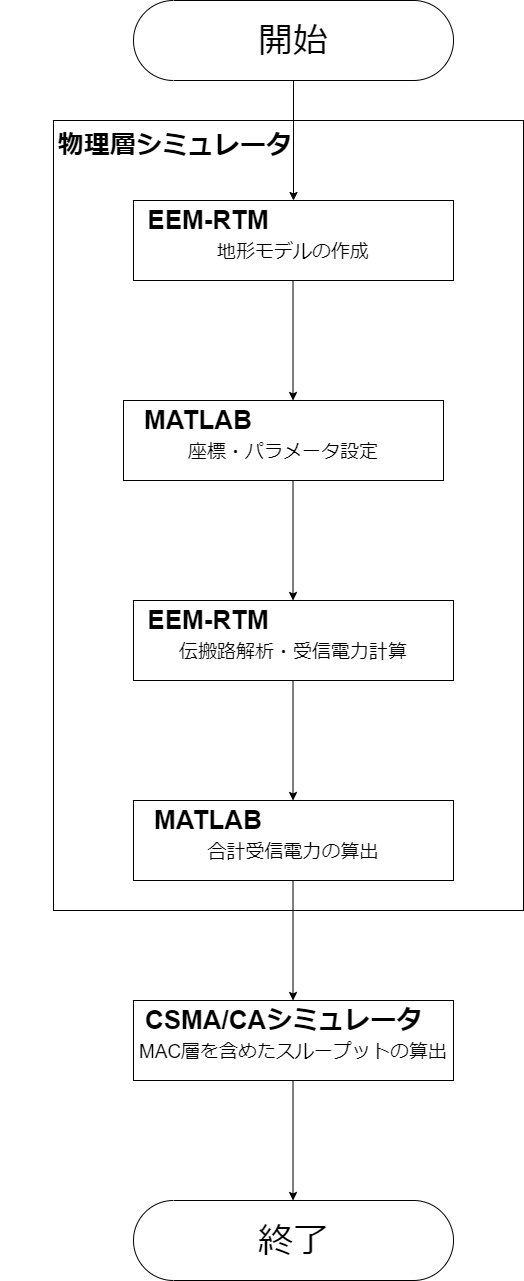
\includegraphics[width=0.35\textwidth]{./assets/cross_simu_flow.drawio.png}
  \caption{提案するクロスレイヤシミュレータのフローチャート}
  \label{fig:cross_simu_flow}
\end{figure}

% ******************************************************
% 評価
% ******************************************************
\clearpage
\section{評価}
\subsection{シミュレーション諸元}

図\ref{fig:topology}に本シミュレーションのトポロジーを,表\ref{tab:sim-base-param}に本シミュレータの諸元を示す.今回のシミュレーションではプロトコルのみを評価するために全ての端末を見通し内として電力を加味せず,同一の伝送レートとして扱った.

\begin{table}[H]
  \centering
  \caption{シミュレーション諸元}
  \label{tab:sim-base-param}
  \begin{tabular}{c|c}
    \hline
    対応規格 & IEEE 802.11a/b/g \\
    \hline
    周波数 & a : 5.2  \,$\mathrm{GHz}$\, \\
    & b/g : 2.4  \,$\mathrm{GHz}$\, \\
    \hline
    ガードインターバル & 800  \,$\mathrm{ns}$\, \\
    \hline
    端末台数 & 1 ~ 80 \, 台\, \\
    \hline
  \end{tabular}
\end{table}

\begin{figure}[H]
  \centering
  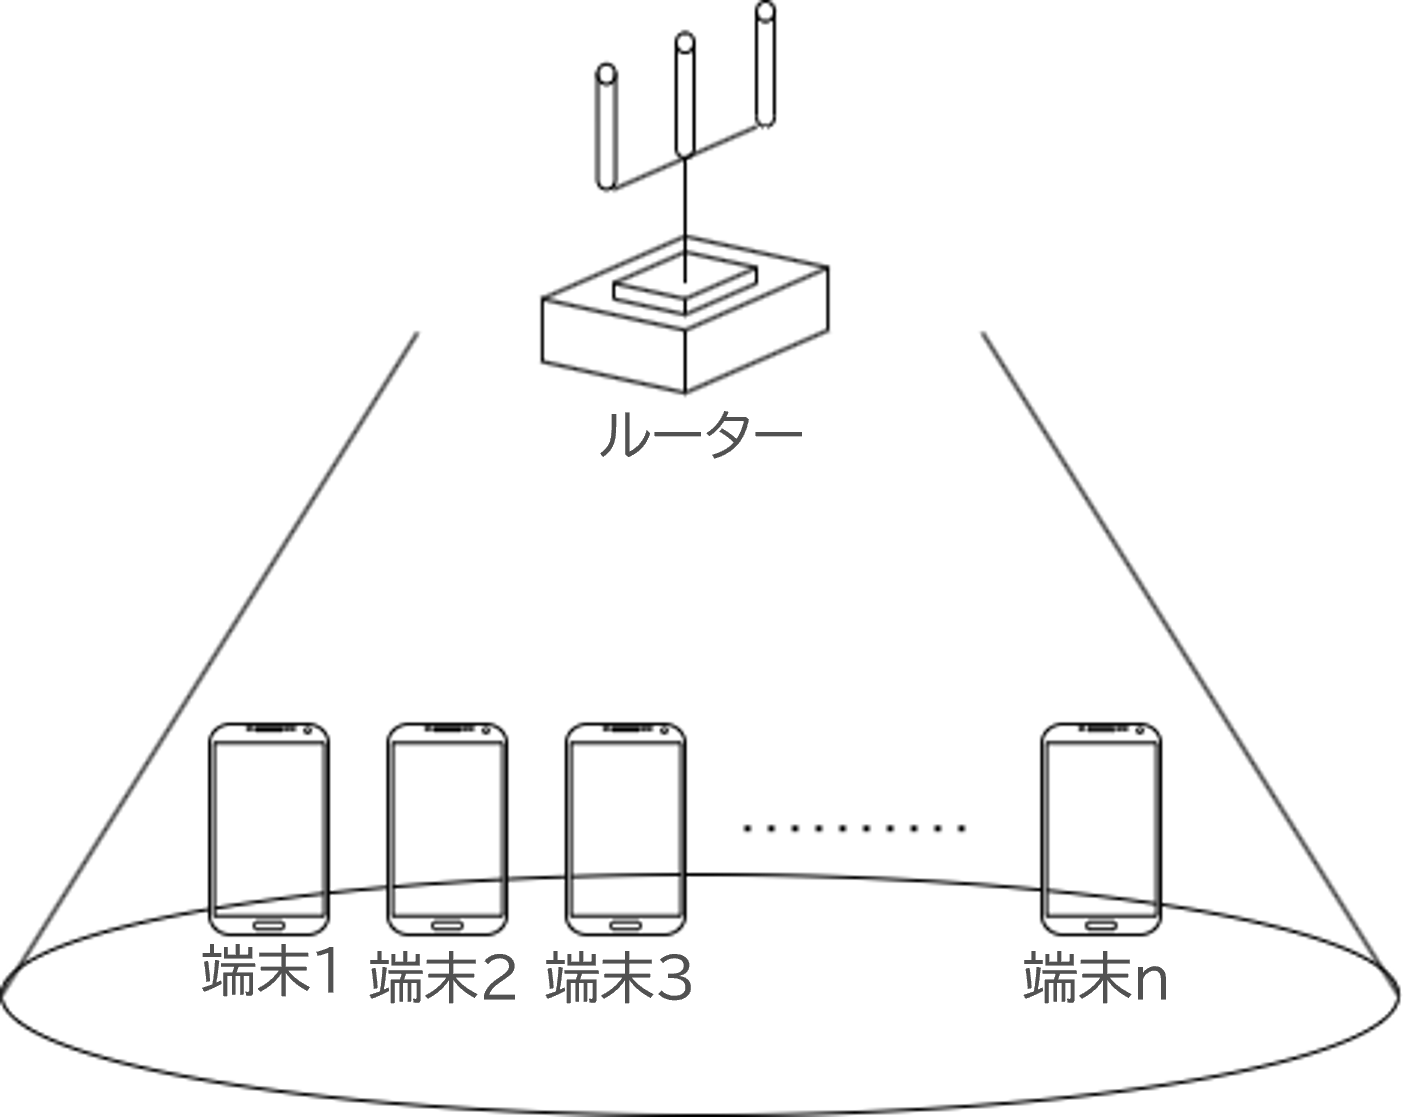
\includegraphics[width=0.8\textwidth]{./assets/topology.png}
  \caption{本シミュレーションのトポロジー}
  \label{fig:topology}
\end{figure}


\clearpage
\subsection{シミュレーション1}
\subsubsection{シミュレーション条件}
今回作成したシミュレータの精度を確認するために,端末数を1台から80台まで10台ずつ変化させ,試行回数1000回としてシミュレーションを行い,理論値\cite{paper}との比較を行った.

表\ref{tab:sim1-param}に本シミュレーションのパラメータを示す.

\begin{table}[H]
  \centering
  \caption{シミュレーション1パラメータ}
  \label{tab:sim1-param}
  \begin{tabular}{c|@{\hspace{1.8em}}l}
    \hline
    パラメータ & 値・例 \\
    \hline
    シミュレーション時間 & 60 \, $\mathrm{s}$\, \\
    モード & \, \,  a \\
    スロット時間 (802.11a) & \, 9  \,$\mathrm{\mu s}$\, \\
    DIFS (802.11a) & 34 \, $\mathrm{\mu s}$\, \\
    SIFS (802.11a) & 16 \, $\mathrm{\mu s}$\, \\
    伝送レート & 24 \, Mbps\, \\
    端末数 & 1~80 \, 台\, \\
    \hline
  \end{tabular}
\end{table}


\subsubsection{結果}

横軸を端末数,縦軸をスループットとした1~80台まで10台ずつ試行回数1000回24\, Mbps固定としてシミュレーションした結果の平均と理論値を図\ref{fig:simulation-result-a}に示す.



\begin{figure}[H]
  \centering
  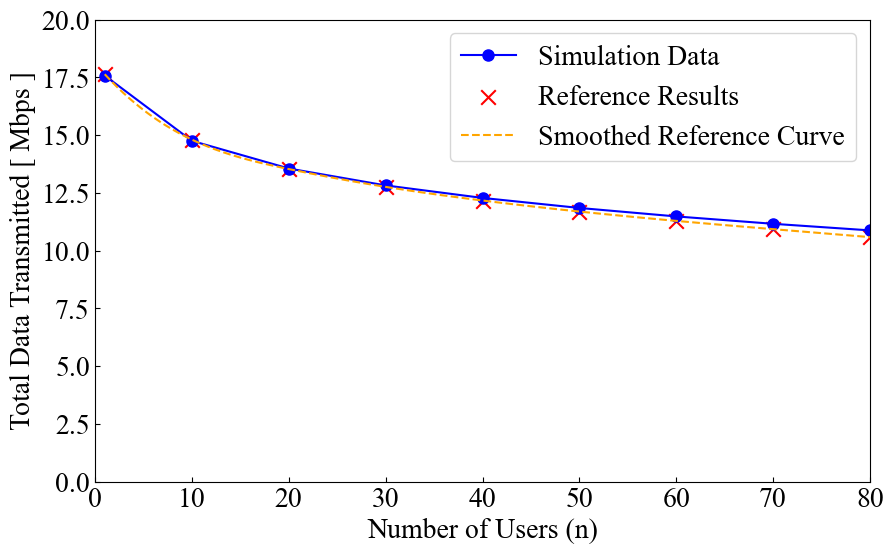
\includegraphics[width=0.9\textwidth]{./assets/g3.png}
  \caption{シミュレーション結果}
  \label{fig:simulation-result-a}
\end{figure}

\subsubsection{考察}

理論値との差が一番大きい端末数が80台の場合でも+2.75\%程度の誤差に収まっていることが確認できる.また,端末数が増加するにつれて理論値との差が徐々に拡大することに対しては,参考とした文献\cite{paper}とのIP(Internet Protocol)レベルとUDPレベルのプロトコル上の違いからくるペイロード長の差などモデル化方法の違いが影響していると考えられる.
以上の結果から,本研究で構築したCSMA/CAベースの無線LANモデルは,理論値に対して概ね一致し,最大でも誤差がおよそ3\%にとどまることが示された.

また,本シミュレータでは文献よりもより現実に則ったモデルを使用しているため,より実際の通信環境に近い状況を再現することができていると考えられる.


\clearpage
\subsection{シミュレーション2}

\subsubsection{シミュレーション条件}
MCS Indexで定義されているIEEE 802.11aに対応する全ての伝送レートに対して,端末数を1台から80台まで10台ずつ変化させ,試行回数1000回としてシミュレーションを行い,24\,Mbpsの場合と同様の傾向を示すか確認を行った.

以下に本シミュレーションのパラメータを示す.

\begin{table}[H]
  \centering
  \caption{シミュレーション2パラメータ}
  \label{tab:sim2-param}
  \begin{tabular}{c|@{\hspace{1.8em}}l}
    \hline
    パラメータ & 値・例 \\
    \hline
    シミュレーション時間 & 60 \, $\mathrm{s}$\, \\
    モード & \, \,  a \\
    スロット時間 (802.11a) & \, 9 \, $\mathrm{\mu s}$\, \\
    DIFS (802.11a) & 34 \, $\mathrm{\mu s}$\, \\
    SIFS (802.11a) & 16 \, $\mathrm{\mu s}$\, \\
    伝送レート & 6~54 \, Mbps\, \\
    端末数 & 1~80 \, 台\, \\
    \hline
  \end{tabular}
\end{table}

\subsubsection{結果}
MCS Indexで定義されているIEEE 802.11aに対応する全ての伝送レートで1~80台まで10台ずつ試行回数1000回としてシミュレーションした結果のを図\ref{fig:simulation-result-mcs-index}に示す.


\begin{figure}[H]
  \centering
  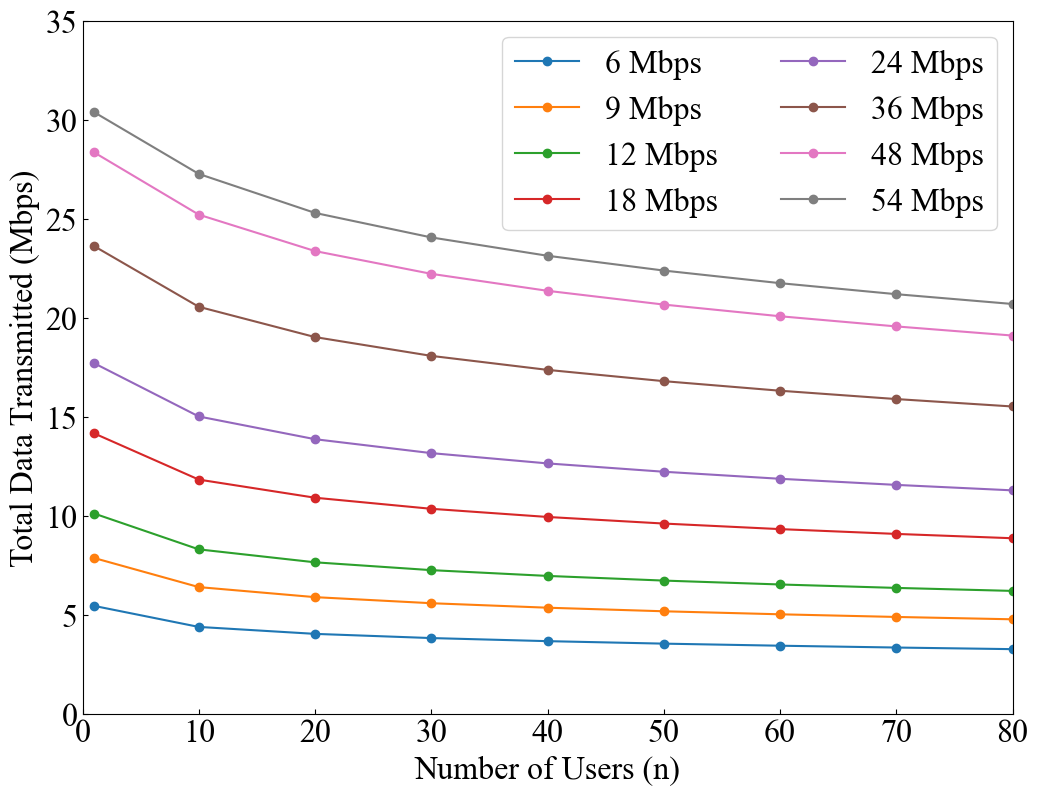
\includegraphics[width=0.9\textwidth]{./assets/mcs_index.png}
  \caption{シミュレーション結果}
  \label{fig:simulation-result-mcs-index}
\end{figure}

\subsubsection{考察}

% 全ての伝送レートの場合で,24Mbpsの場合と同様の傾向を示すことが確認できた.

IEEE 802.11aにおけるMCS Indexで定義されている全ての伝送レートにおいて24\,Mbpsの場合と同様に端末数の増加に伴いスループットが減少する傾向が見られた.

伝送レートが高いほど端末数が増えるにつれスループットが低下する傾向が見られるが,これはデータ送信に必要な時間が短縮され,フレーム間隔やバックオフ時間の相対的に増加するためであると考えられる.また,フレーム衝突による再送制御の頻度が増えると,バックオフ時間の増加に伴うオーバーヘッドが全体の性能に深刻な影響を与えることが分かる.低い伝送レートでは端末数が端末数が多くても比較的スループットの低下幅が小さい傾向が見られる.これは,低レートではデータ送信に必要な時間が長くなるため,フレーム間隔やバックオフ時間が相対的に小さくなるためであると考えられる.

これらのことから,本シミュレータでは実際の無線LANにおけるMAC層のプロトコルの動作を模擬したシミュレータを構築することができたと考えられる.

% ******************************************************
% 結論
% ******************************************************
\clearpage
\section{結論}
\subsection{まとめ}
本研究では,無線LANにおけるクロスレイヤ評価を目的として,物理層からMAC層までを考慮したシミュレータの開発を行った.このシミュレータは電波伝搬特性を考慮した物理層シミュレータと連携を行い,MAC層の動作を評価することができる.

本シミュレータと理論値を24\,Mbpsの場合で比較した評価では,差が最大でも約2.75\%となり,本シミュレータの有効性を示すことができた.また,IEEE 802.11aにおけるMCS Indexで定義されている全ての伝送レートでシミュレーションを行い,同様の傾向があることを確認した.

これらの結果から,無線LANにおけるクロスレイヤ評価のために物理層シミュレータと組み合わせることで,MAC層のプロトコルの動作を評価することができるシミュレータを実現することができたと考えられる.



\subsection{今後の課題}
本シミュレータの今後の課題については以下が挙げられる.

\begin{enumerate}
  \item \texttt{送信間隔}\\送信間隔を連続送信からポアソン分布にすることでより現実に即した送信間隔を再現する
  \item \texttt{距離の概念の導入}\\\texttt{User}クラスに距離や位置の概念を導入し,その情報を踏まえて各端末を個別の伝送レートで評価する
  \item \texttt{キャプチャ効果の導入}\\各端末やアクセスポイントの位置情報を踏まえて受信時のSNRを考慮し,衝突時でもフレームの複合が可能となるキャプチャ効果を導入することで,より実環境に近い通信環境を再現する
\end{enumerate}


% ******************************************************
% 参考文献
% ******************************************************
\clearpage
\addcontentsline{toc}{section}{参考文献}
\begin{thebibliography}{99}
  \bibitem{11std}IEEE 802.11 Standard for Local and Metropolitan Area
  Networks, “Part 11: Wireless LAN Medium Access Control (MAC) and Physical Layer (PHY) Specifications,”  IEEE Std. 802.11, Mar. 2012.
\bibitem{midori}守倉正博, 久保田周治, 『インプレス標準教科書シリーズ 改訂三版802.11 高速無線LAN教科書』, 株式会社インプレスコミュニケーションズ, 2016年
\bibitem{paper}Y. Morino, T. Hiraguri, H. Yoshino, K. Nishimori, T. Matsuda, ``A Novel Collision Avoidance Scheme Using Optimized Contention Window in Dense Wireless LAN Environments*'' \, \textit{IEICE TRANS. COMMUN.}, VOL.E99-B, NO.11 NOVEMBER 2016
\bibitem{book1}西森健太郎,平栗健史,『MIMOからMassive MIMOを用いた伝送技術とクロスレイヤ評価手法』, コロナ社, 2017年.
\bibitem{book2}設樂勇, 平栗健史, 谷口諒太郎, 西森健太郎, 『レイトレースを用いた3次元クロスレイヤシミュレータの開発』, 社団法人 電子情報通信学会 信学技報
\end{thebibliography}


\end{document}